\section{Statikus struktúra diagram}
\begin{figure}[H] 
\centering 
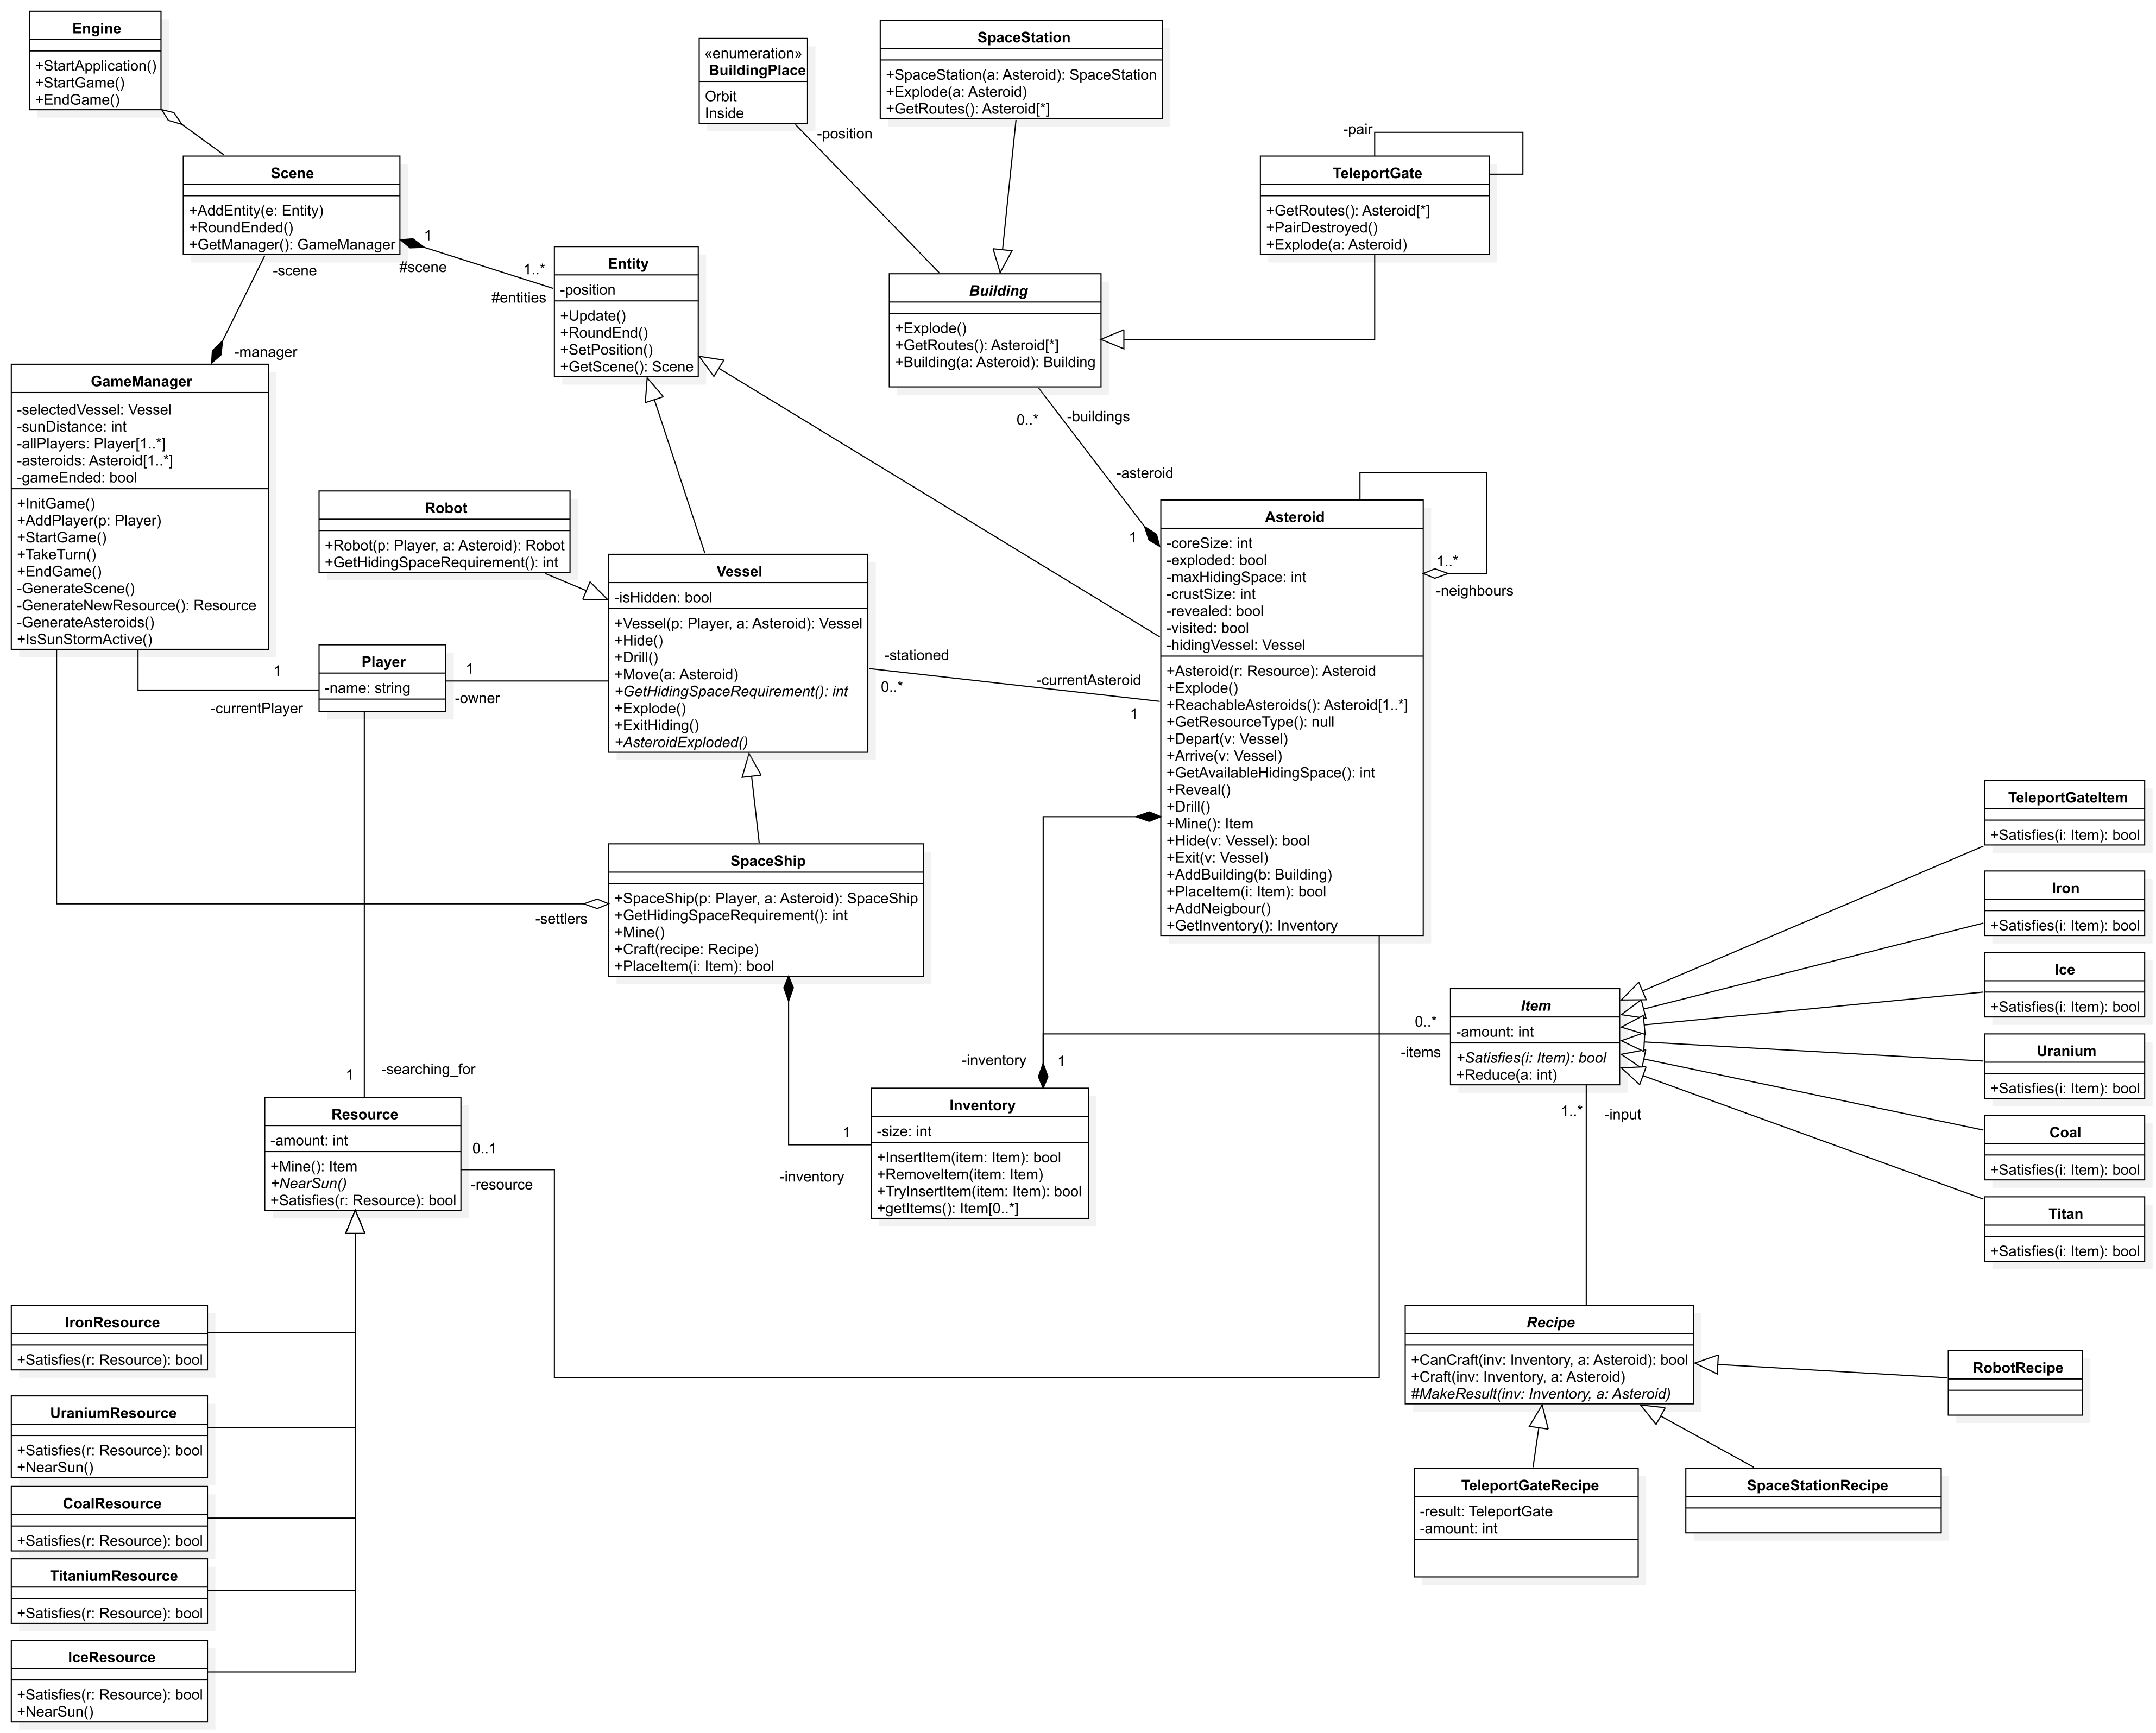
\includegraphics[width=1\textwidth]{docs/3_Project/svg/Design Model!Classes_1.png} 
\end{figure} 

\section{Szekvencia diagramok}
\begin{figure}[H] 
\centering 
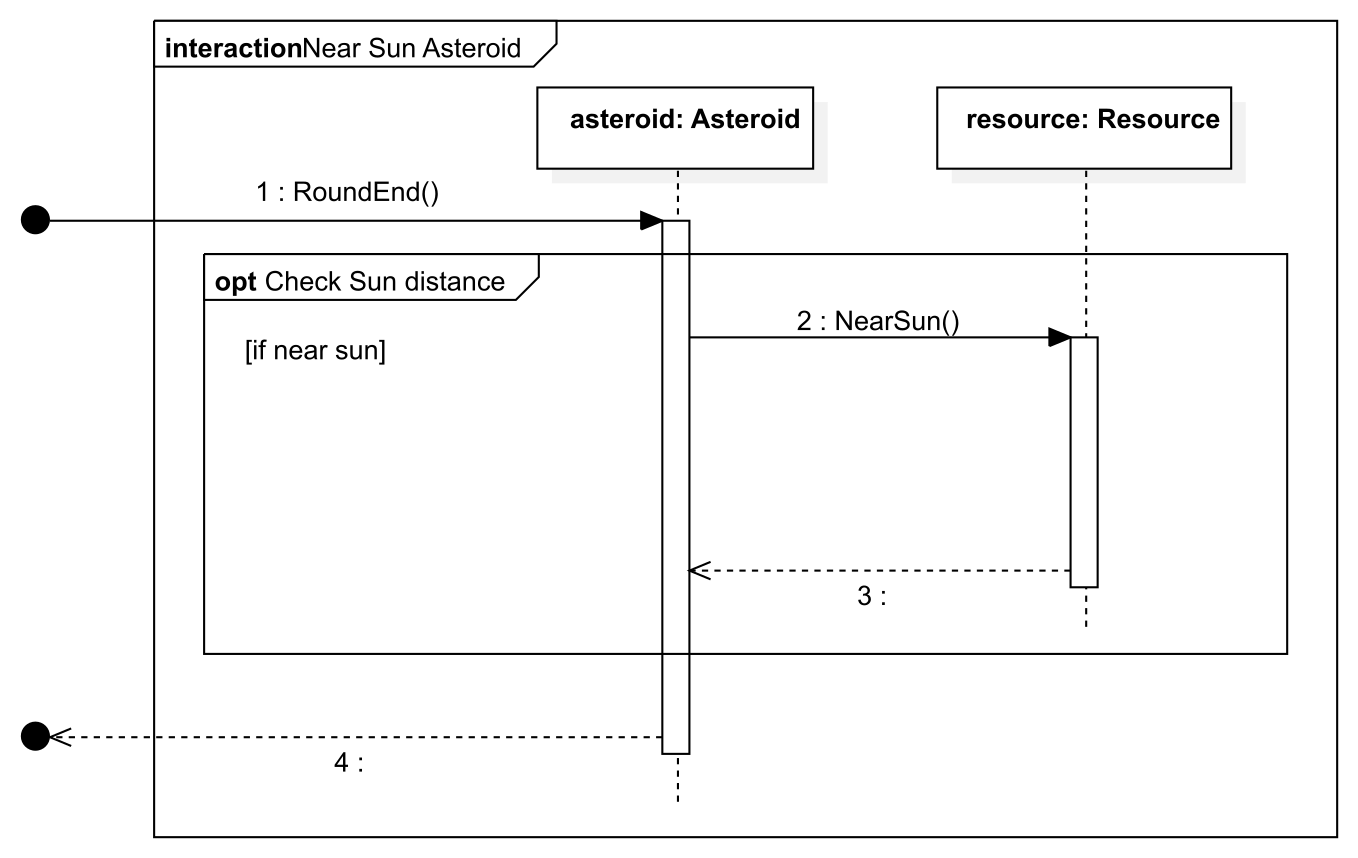
\includegraphics[width=1\textwidth]{docs/3_Project/svg/Design Model!Sun Distance!Asteroid near sun!Near Sun Asteroid_6.png} 
\caption{Egy aszteroidának jelezzük a kör végén, hogy napközelben van.} 
\end{figure} 

\begin{figure}[H] 
\centering 
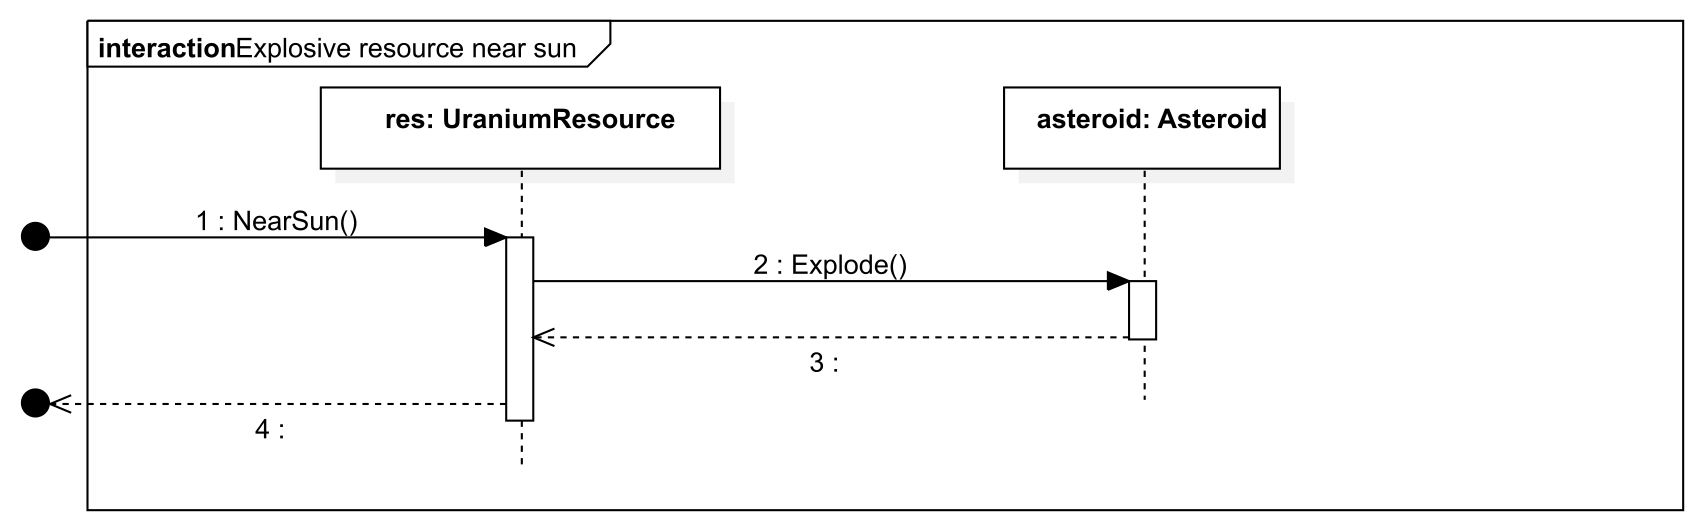
\includegraphics[width=1\textwidth]{docs/3_Project/svg/Design Model!Sun Distance!Resource Explosion!Explosive resource near sun_7.png} 
\caption{Ha napközelben van az aszteroida átfúrt kéreggel, akkor a radioaktív nyersanyag reagálni fog, az aszteroida felrobban.} 
\end{figure} 

\begin{figure}[H] 
\centering 
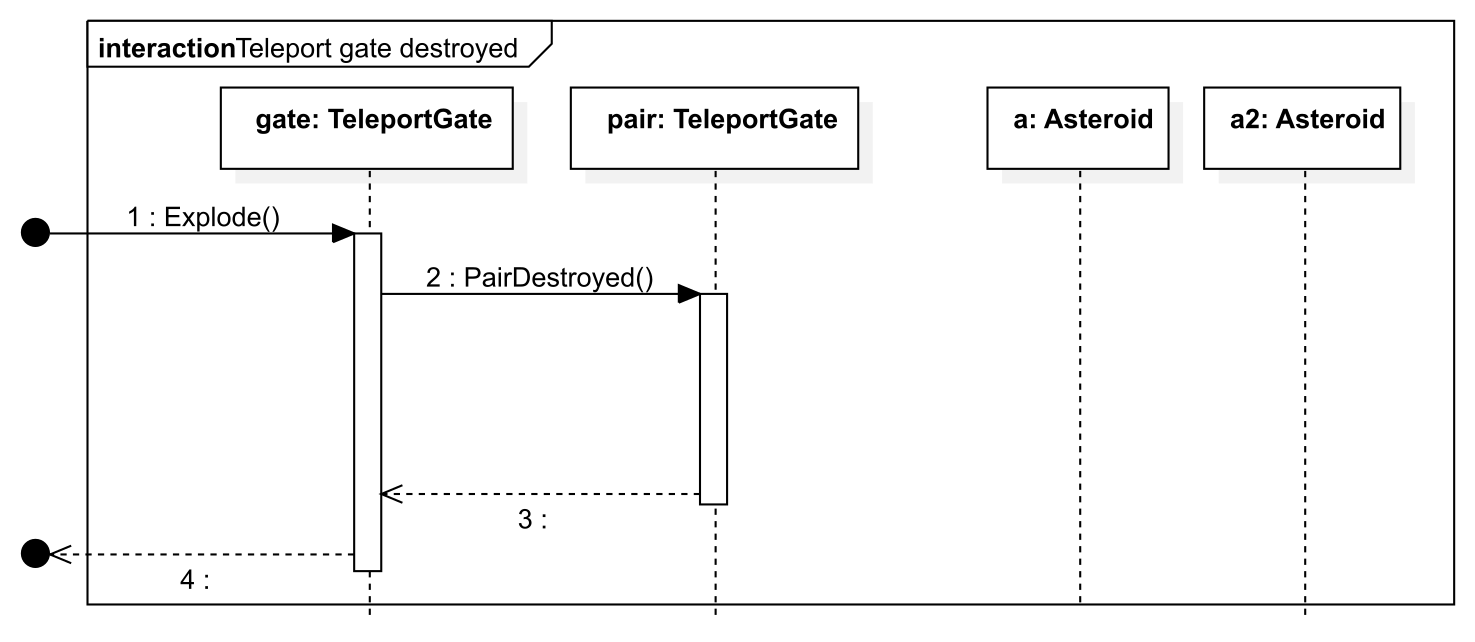
\includegraphics[width=1\textwidth]{docs/3_Project/svg/Design Model!Sun Distance!Teleport gate destroyed!Teleport gate destroyed_8.png} 
\caption{Ha felrobban az aszteroida amin a teleportkapu van, akkor az értesíti a párját is a robbanásról, így mindkettő megsemmisül.} 
\end{figure} 

\begin{figure}[H] 
\centering 
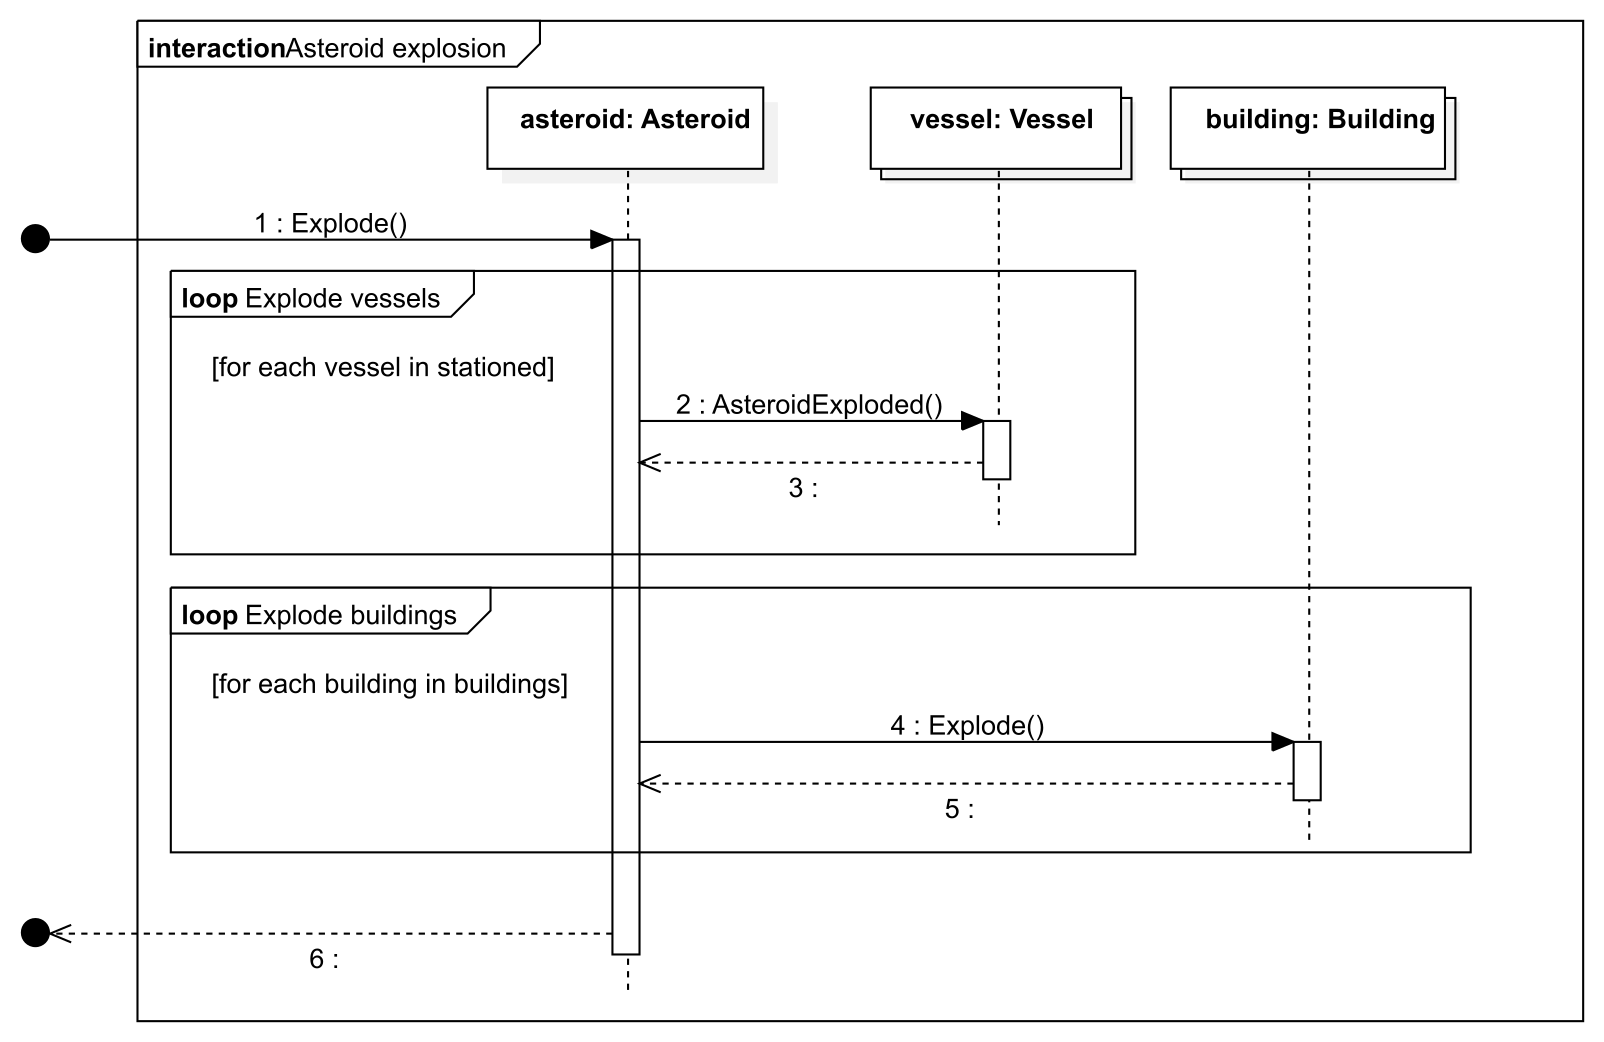
\includegraphics[width=1\textwidth]{docs/3_Project/svg/Design Model!Sun Distance!Asteroid explosion!Asteroid explosion_9.png} 
\caption{Ha felrobban az aszteroida, akkor értesítjük az összes épületet és űrjárművet a robbanásról.} 
\end{figure} 

\begin{figure}[H] 
\centering 
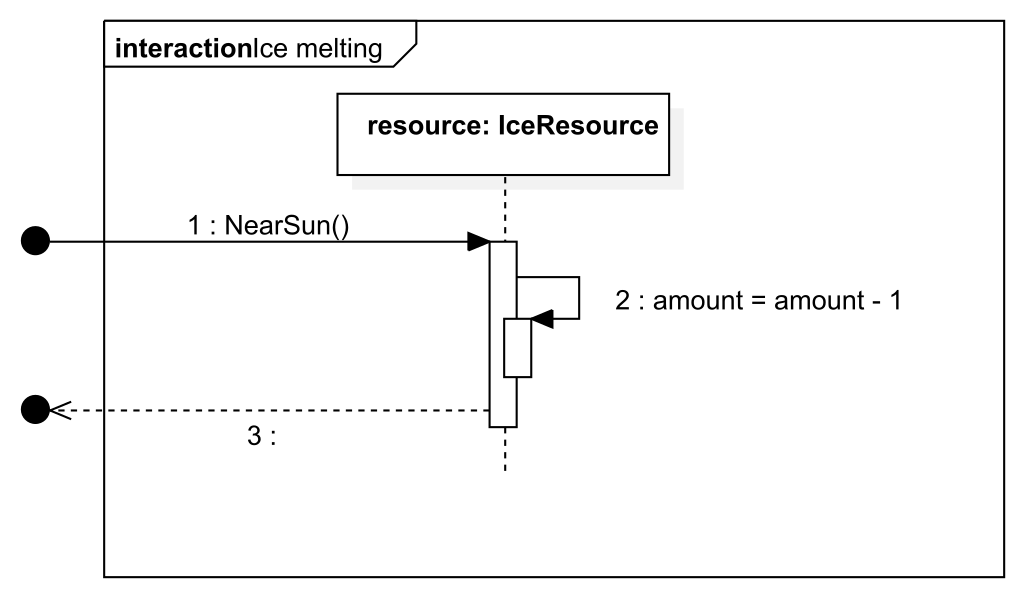
\includegraphics[width=1\textwidth]{docs/3_Project/svg/Design Model!Sun Distance!Ice melting!Ice melting_10.png} 
\caption{Ha napközelben van az aszteroida átfúrt kéreggel, akkor a szublimáló nyersanyag reagálni fog és körönként csökken a mennyisége.} 
\end{figure} 

\begin{figure}[H] 
\centering 
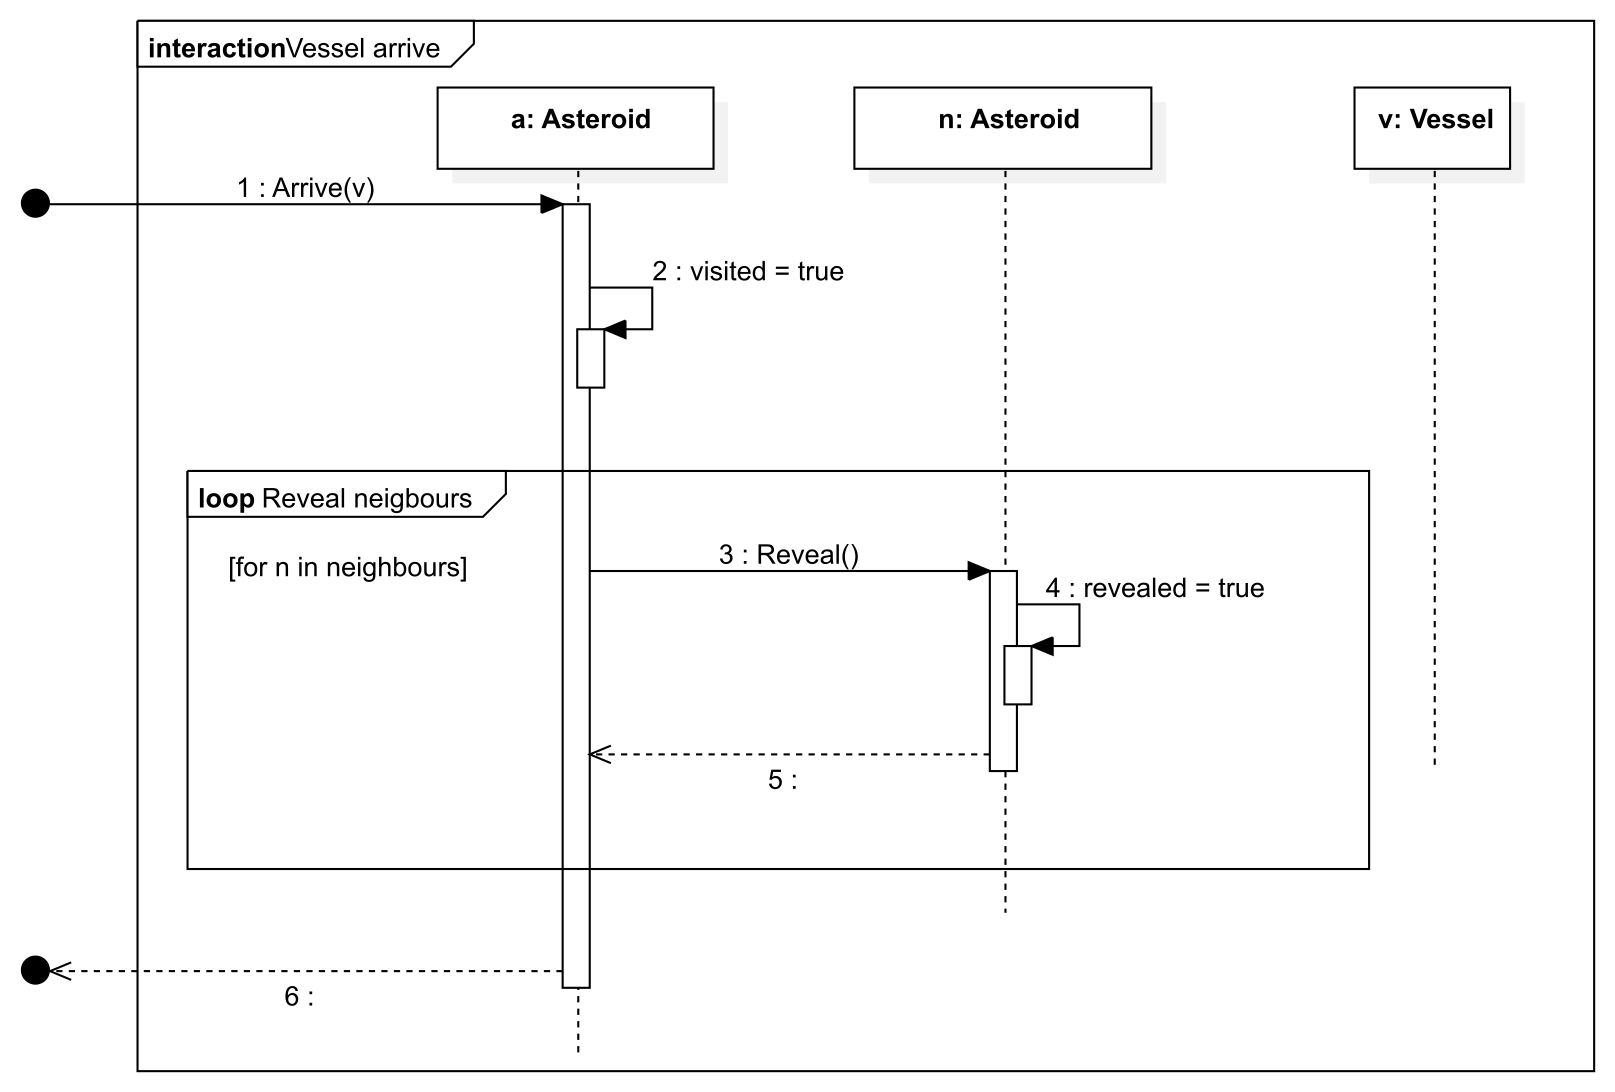
\includegraphics[width=1\textwidth]{docs/3_Project/svg/Design Model!Vessel Actions!Vessel arrive!Vessel arrive_11.png} 
\caption{Amikor az úrjűrmű megérkezik egy aszteroidára, akkor az felfedi a szomszédos aszteroidákat is, ha nem lettek volna már felfedve.} 
\end{figure} 

\begin{figure}[H] 
\centering 
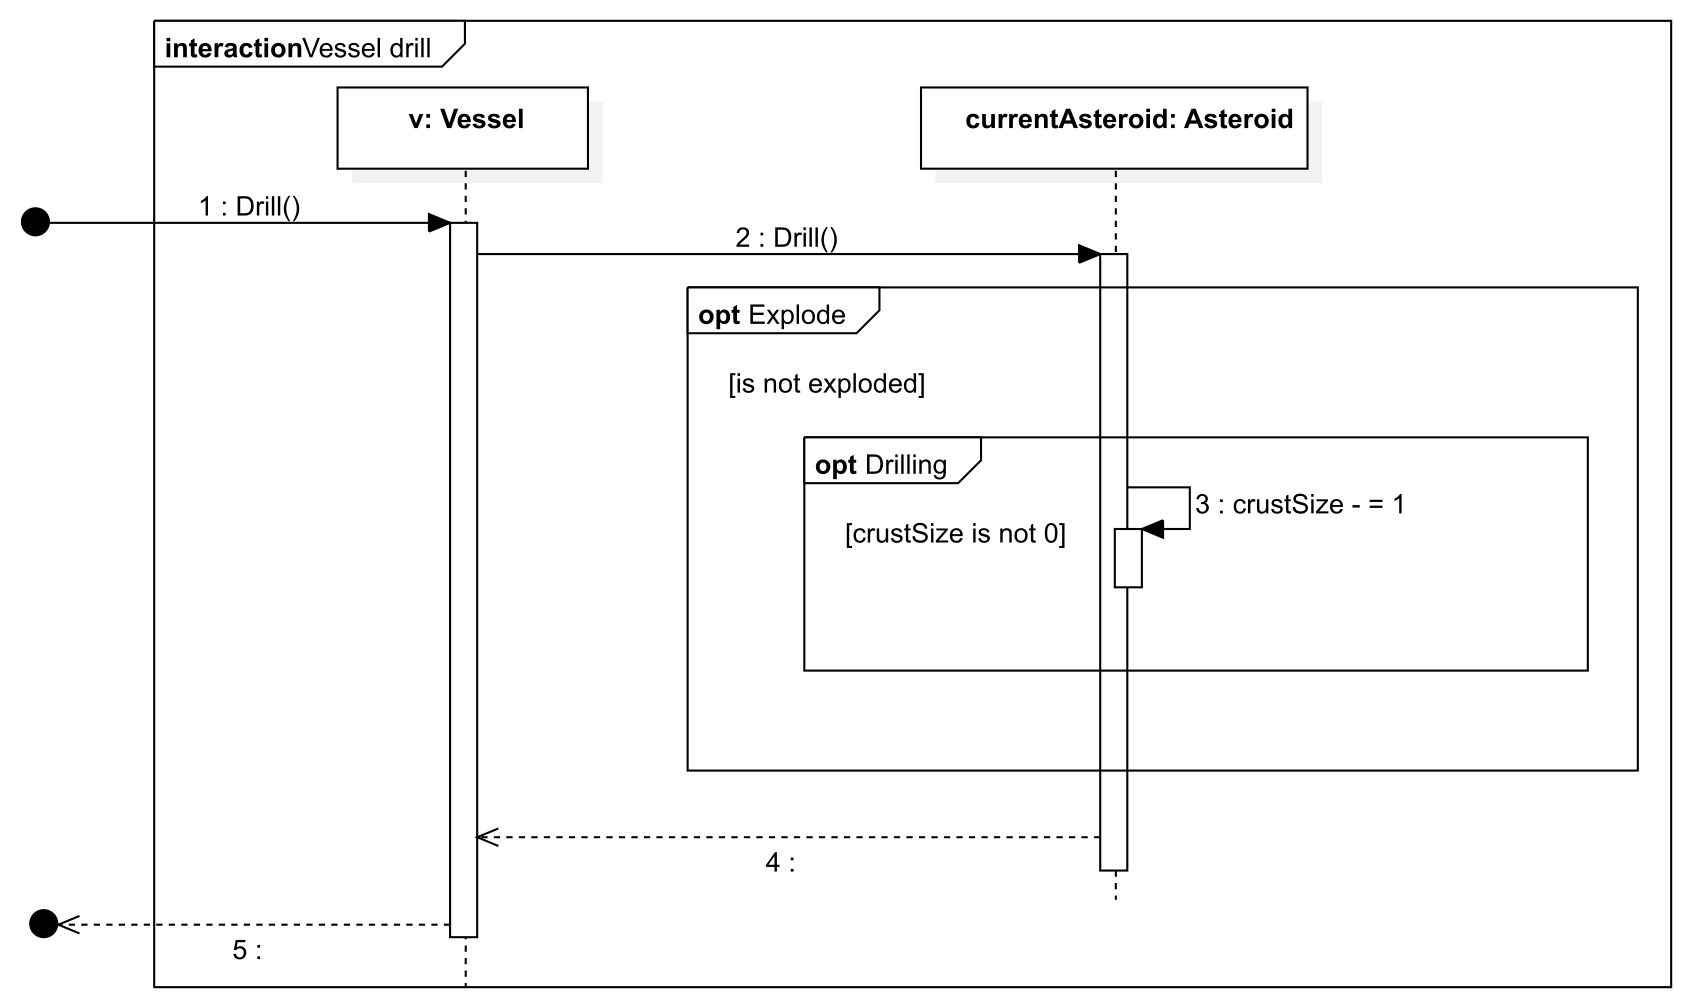
\includegraphics[width=1\textwidth]{docs/3_Project/svg/Design Model!Vessel Actions!Vessel drill!Vessel drill_12.png} 
\caption{Csak akkor tudunk mélyíteni a kérgen, ha nem robbant fel már az aszteroida és ha nem fúrtunk már át a lérgen.} 
\end{figure} 

\begin{figure}[H] 
\centering 
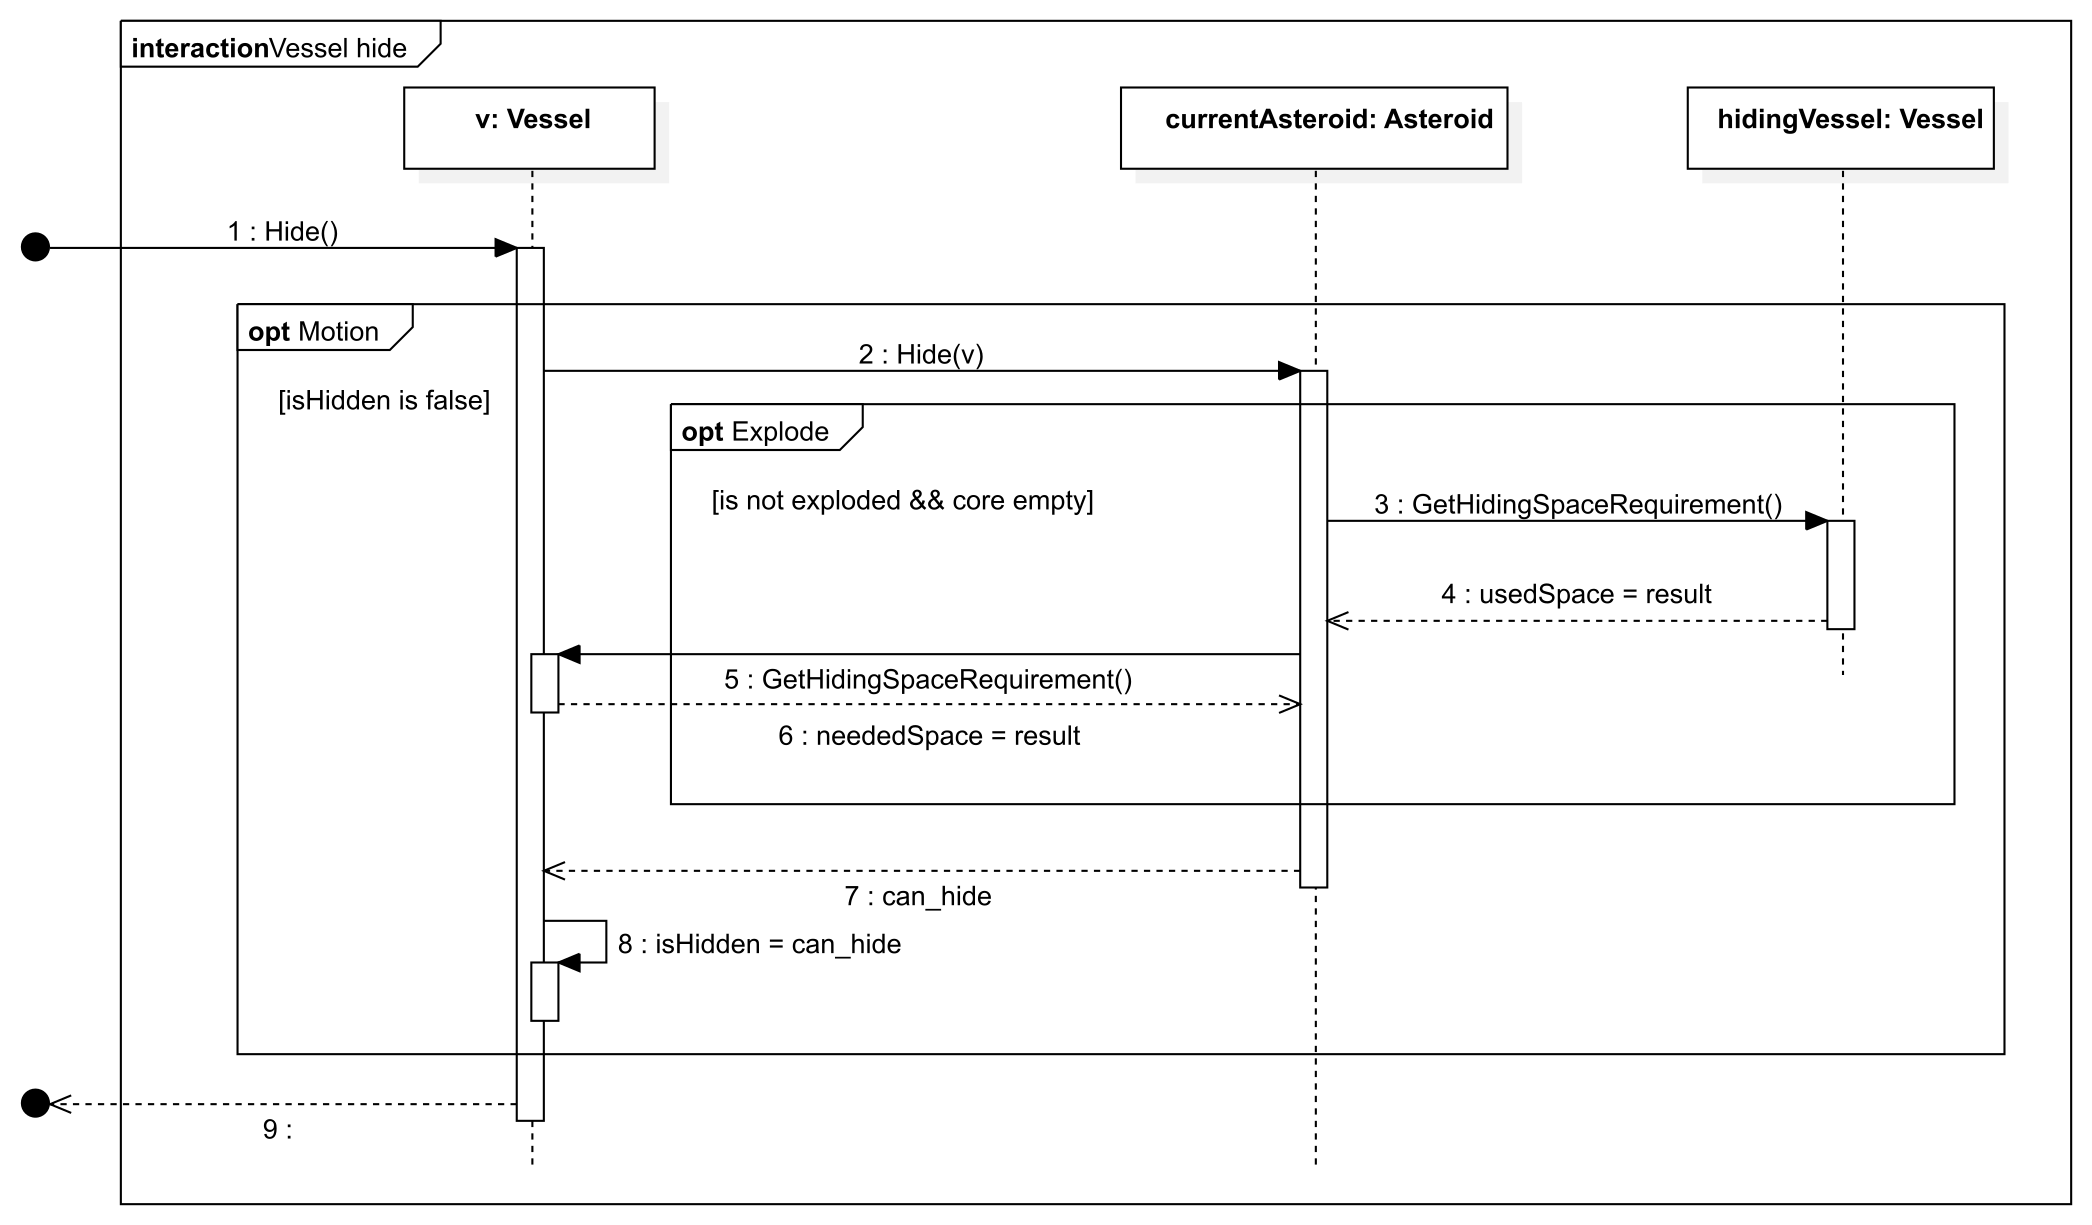
\includegraphics[width=1\textwidth]{docs/3_Project/svg/Design Model!Vessel Actions!Vessel hide!Vessel hide_13.png} 
\caption{Egy űrjármű elbújik. A telepesek helyet foglalnak az aszteroidában, amikor elbújnak, ezért csak korlátozott számú telepes bújhat el.} 
\end{figure} 

\begin{figure}[H] 
\centering 
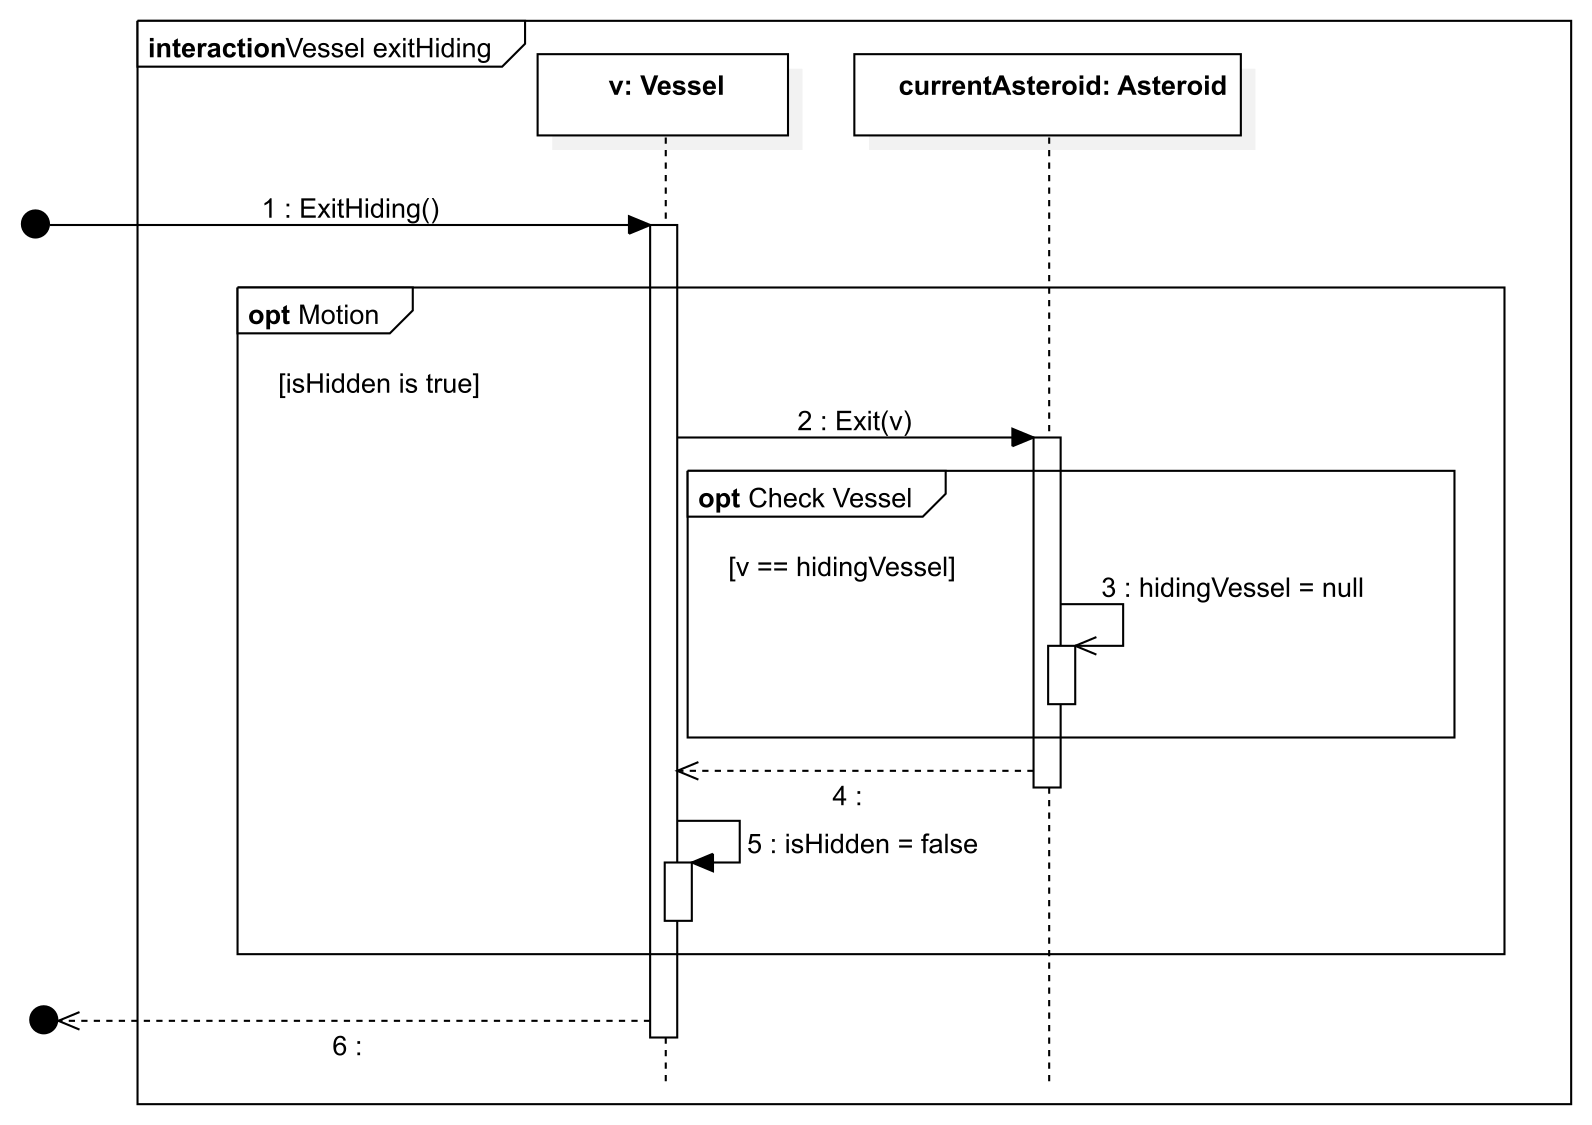
\includegraphics[width=1\textwidth]{docs/3_Project/svg/Design Model!Vessel Actions!Vessel exitHiding!Vessel exitHiding_14.png} 
\caption{Egy űrjármű kijön a rejtekhelyéről.} 
\end{figure} 

\begin{figure}[H] 
\centering 
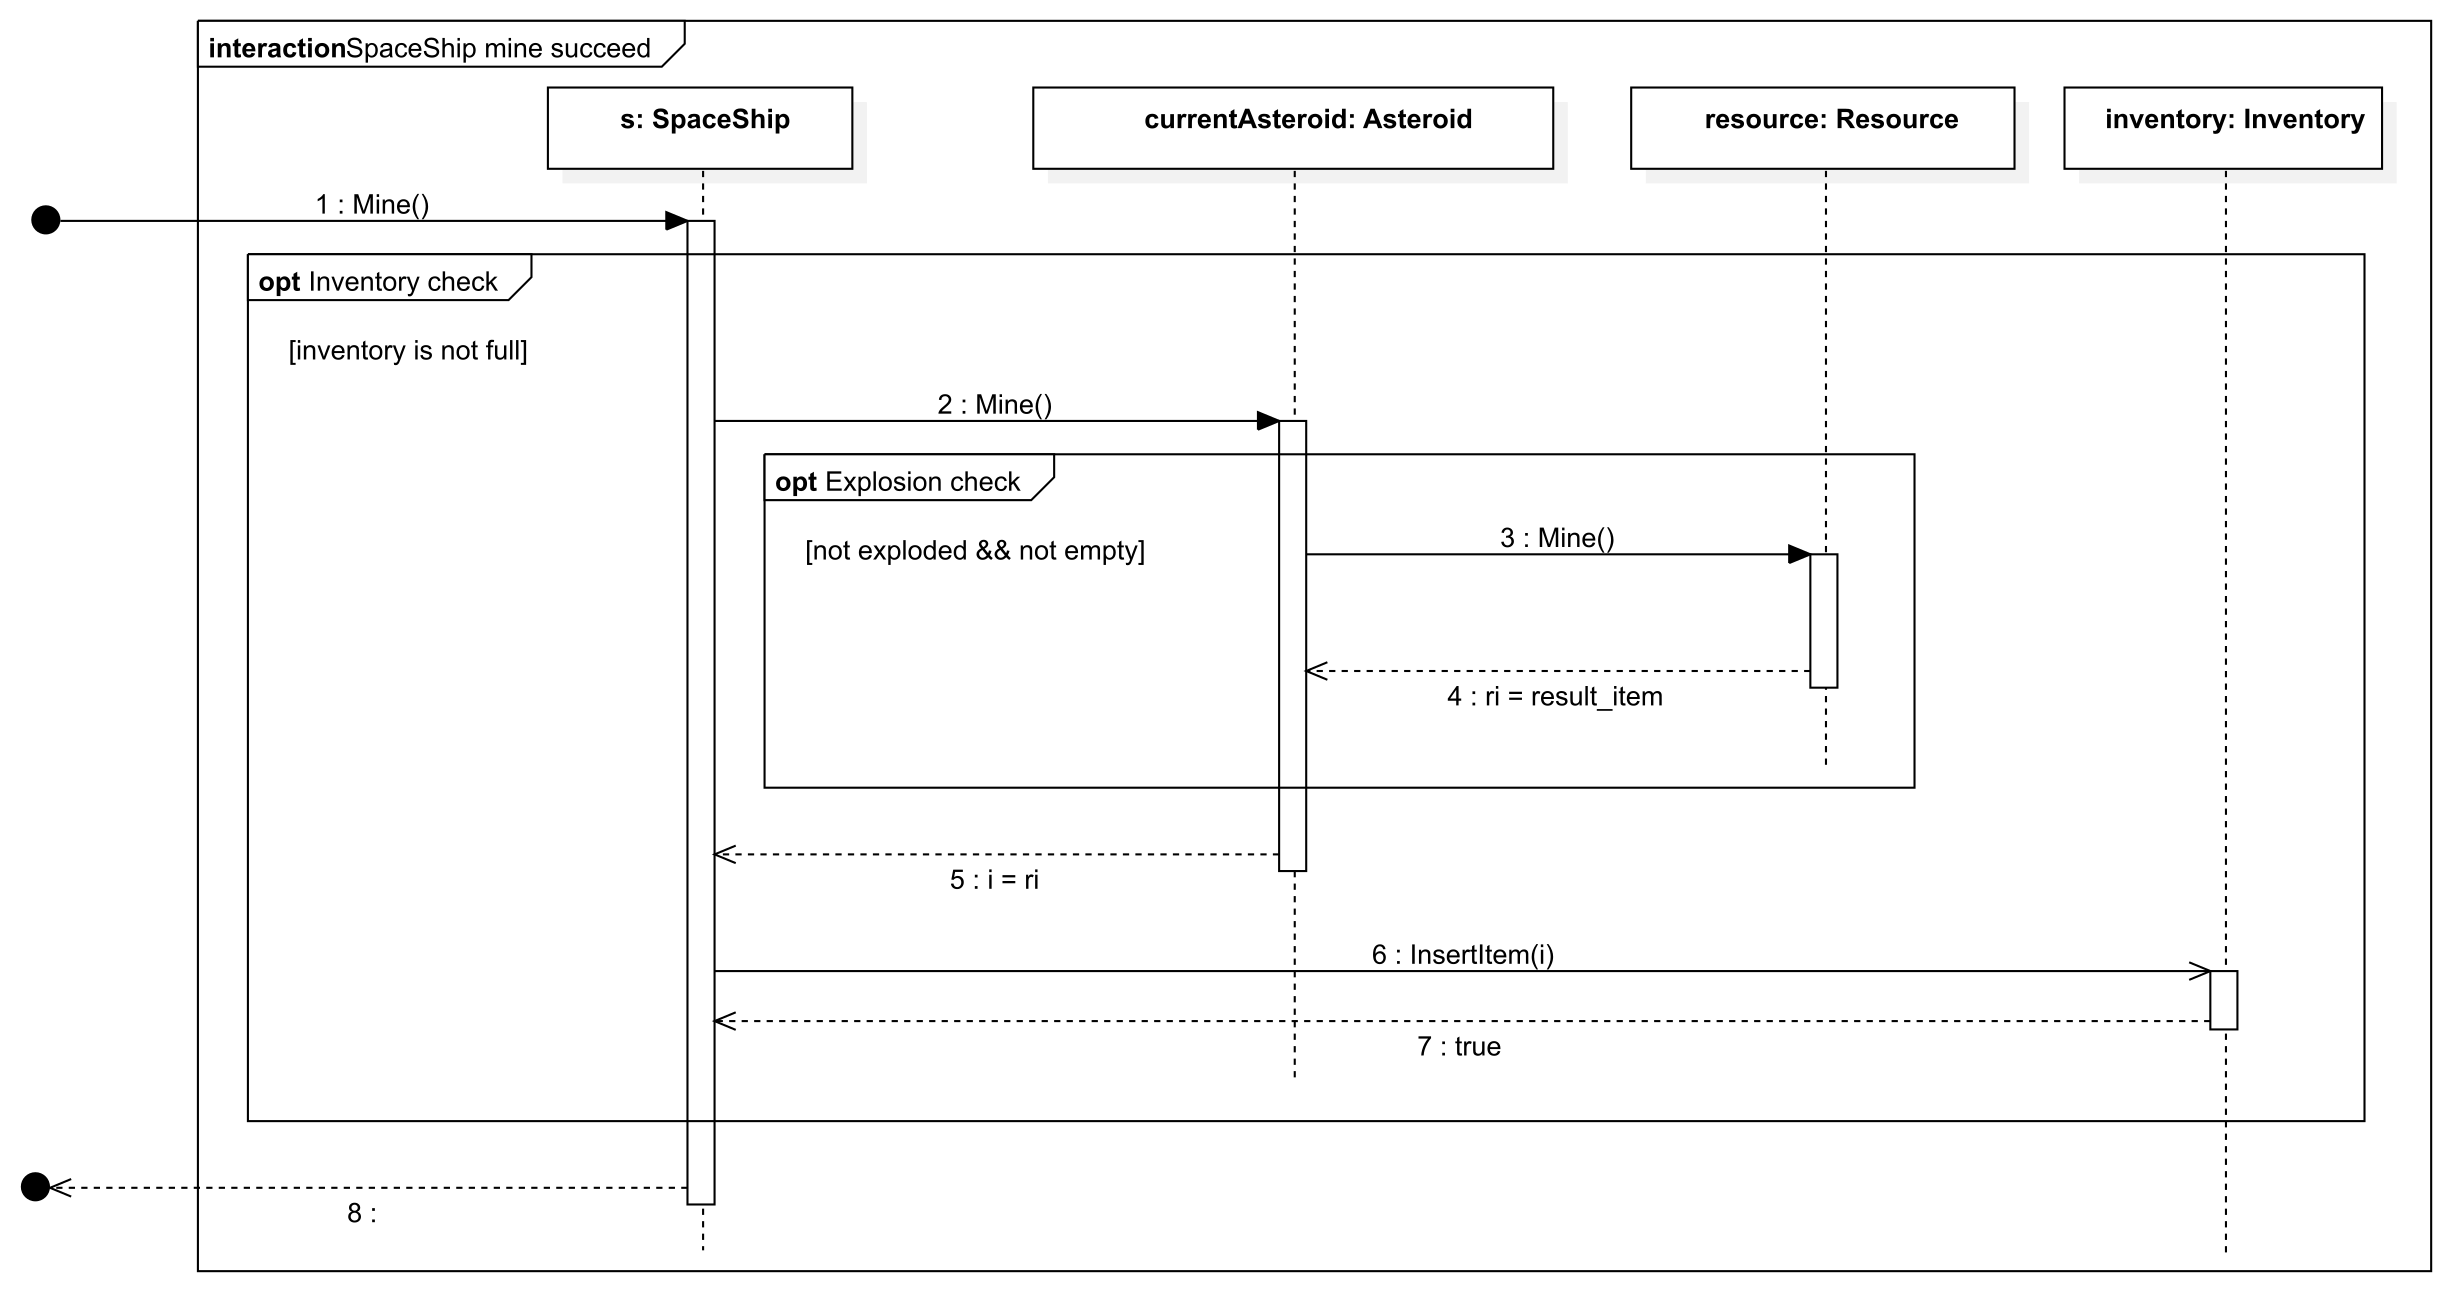
\includegraphics[width=1\textwidth]{docs/3_Project/svg/Design Model!Vessel Actions!SpaceShip mine succeed!SpaceShip mine succeed_15.png} 
\caption{A telepesek csak akkor tudnak bányászni a nyersanyagból, ha átfúrták a kérget, illetve, ha van mit.} 
\end{figure} 

\begin{figure}[H] 
\centering 
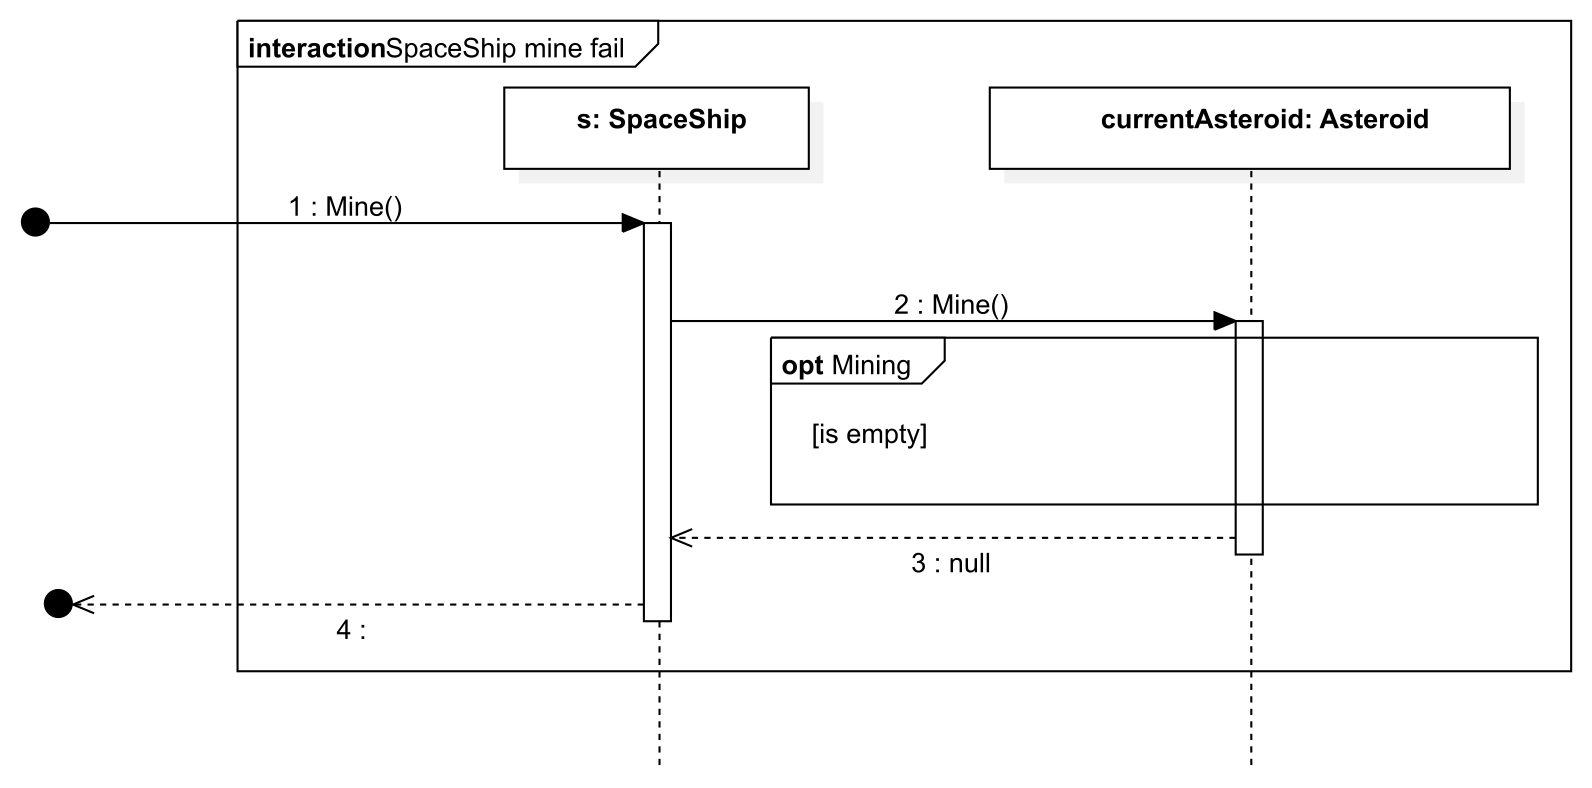
\includegraphics[width=1\textwidth]{docs/3_Project/svg/Design Model!Vessel Actions!SpaceShip mine fail!SpaceShip mine fail_16.png} 
\caption{Ha nincs nem kinyert nyersanyag az aszteroidában, akkor nem lehet nyersanyagot kibányászni belőle.} 
\end{figure} 

\begin{figure}[H] 
\centering 
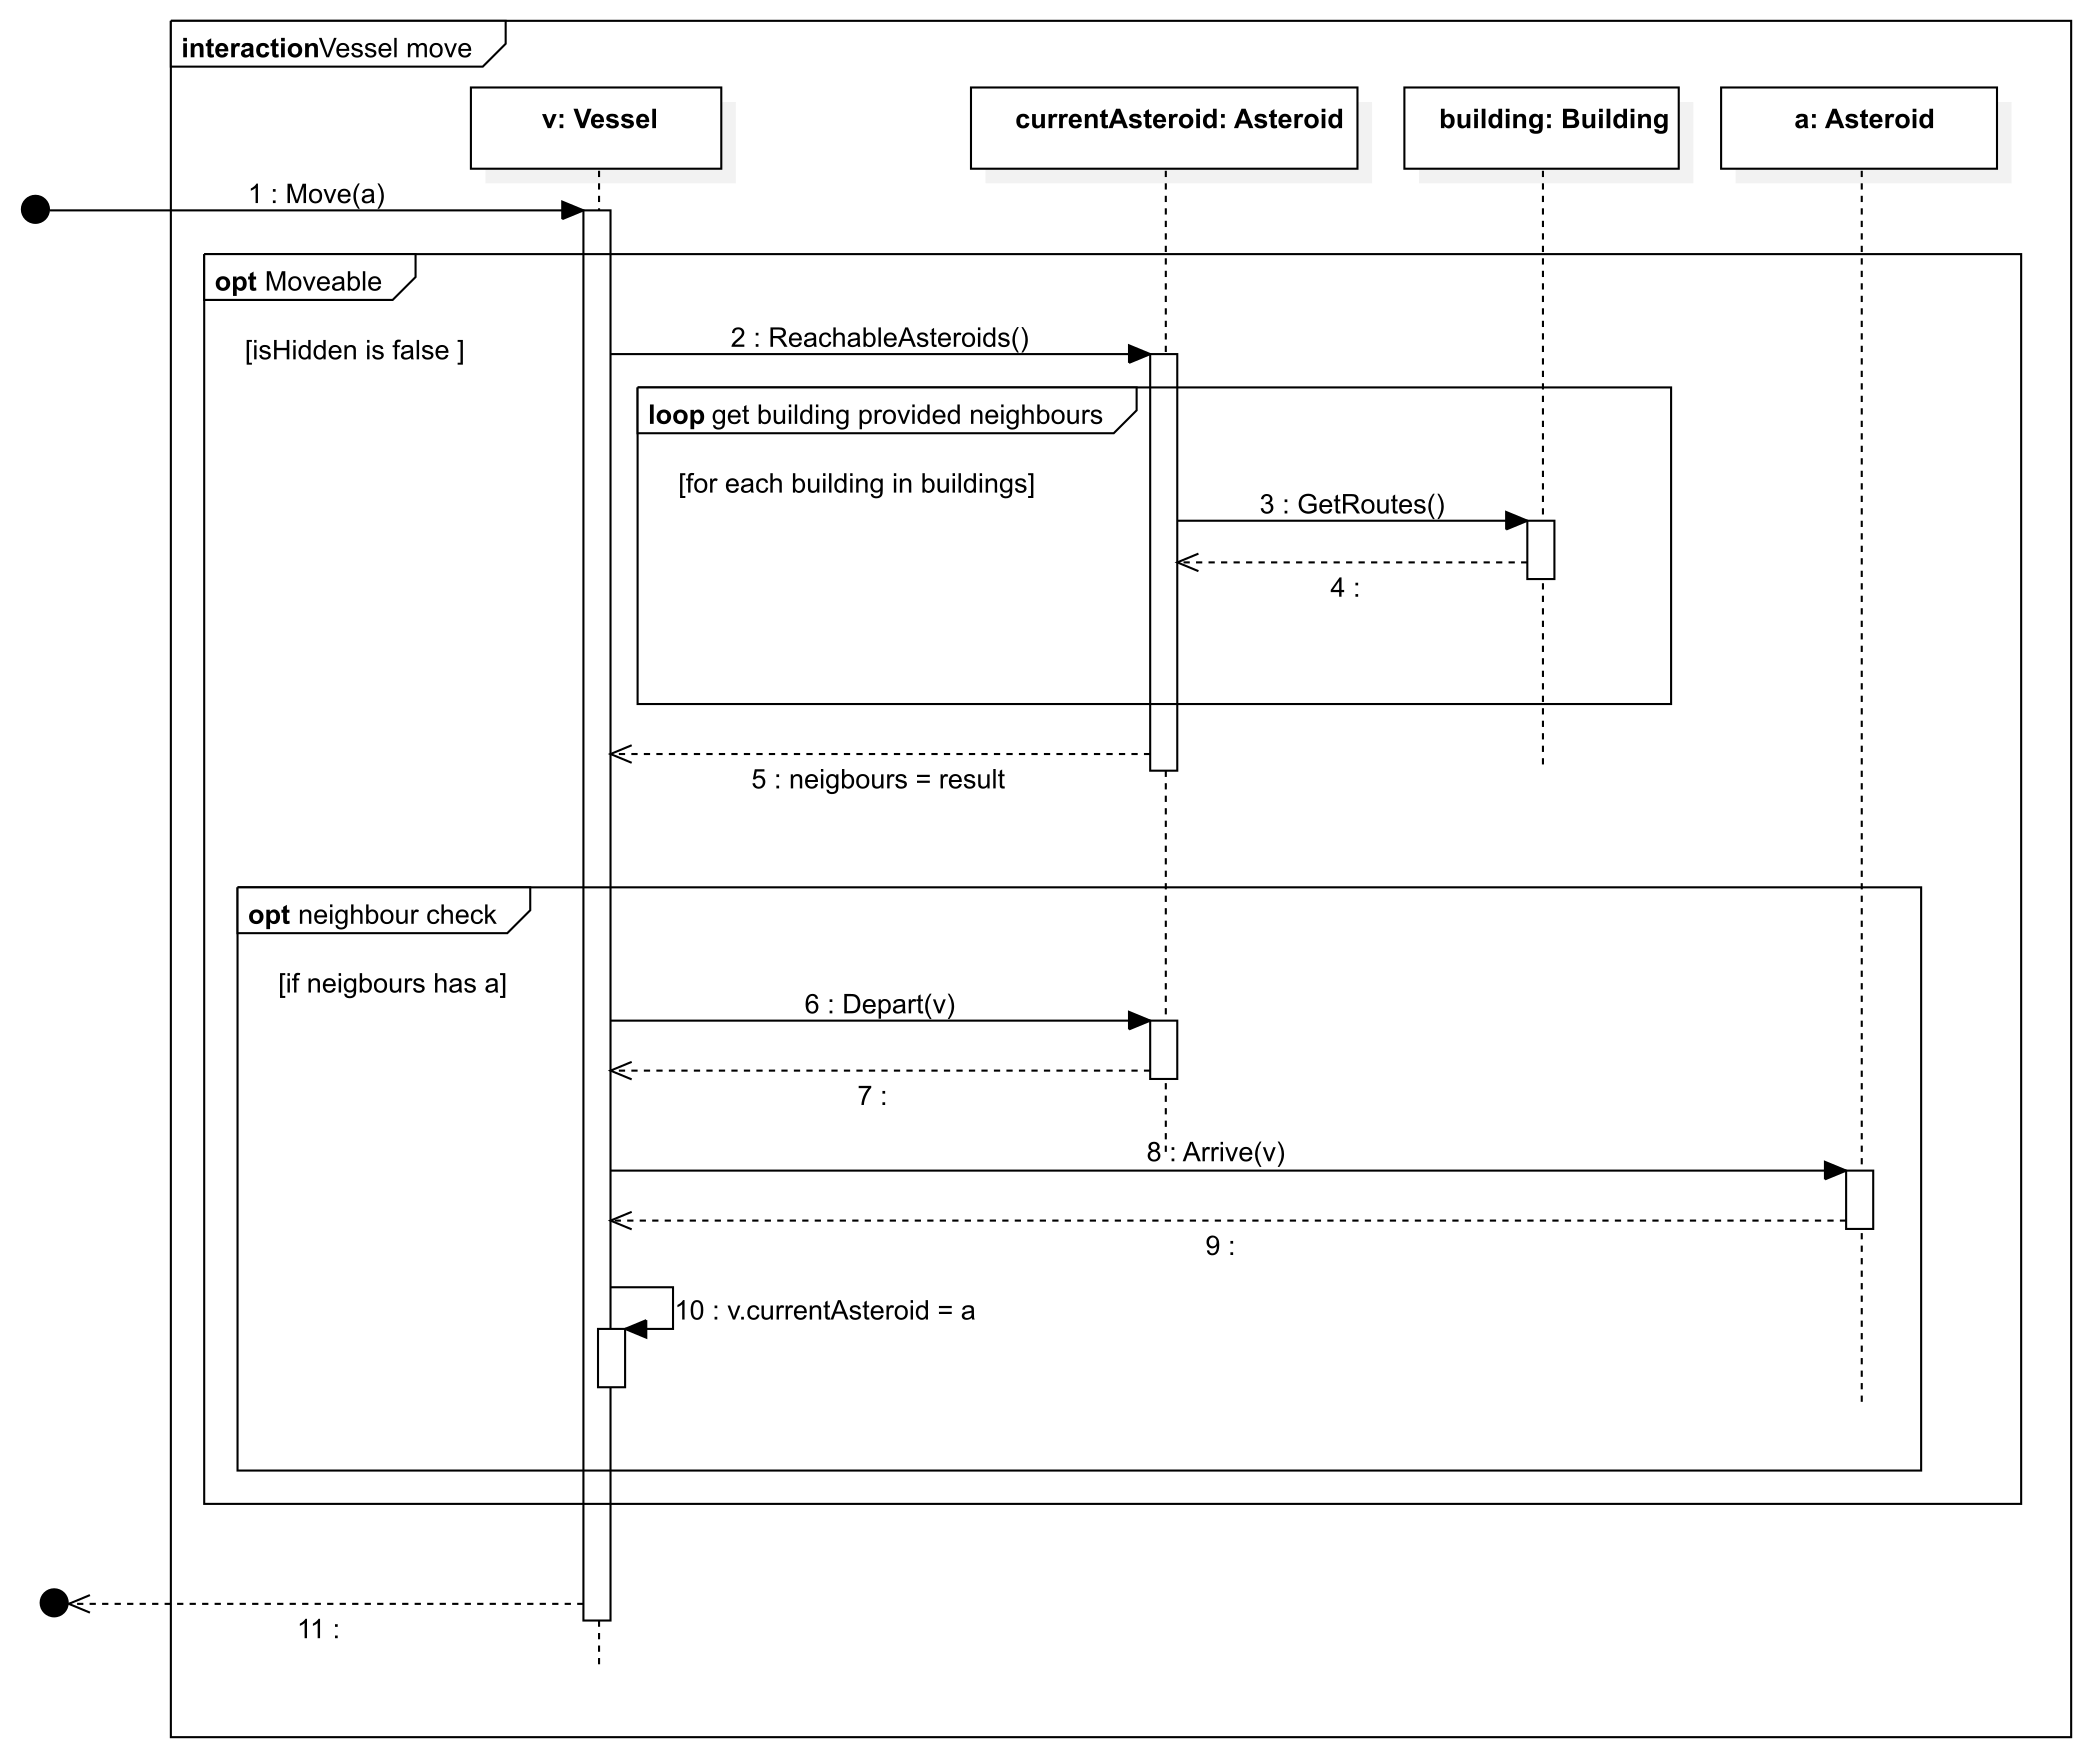
\includegraphics[width=1\textwidth]{docs/3_Project/svg/Design Model!Vessel Actions!Vessel move!Vessel move_17.png} 
\caption{Egy űrjármű mozogni szeretne. Ezt csak akkor tudja megtenni, ha a célpont szomszdédos, illetve ha nincs elbújva a jármű.} 
\end{figure} 

\begin{figure}[H] 
\centering 
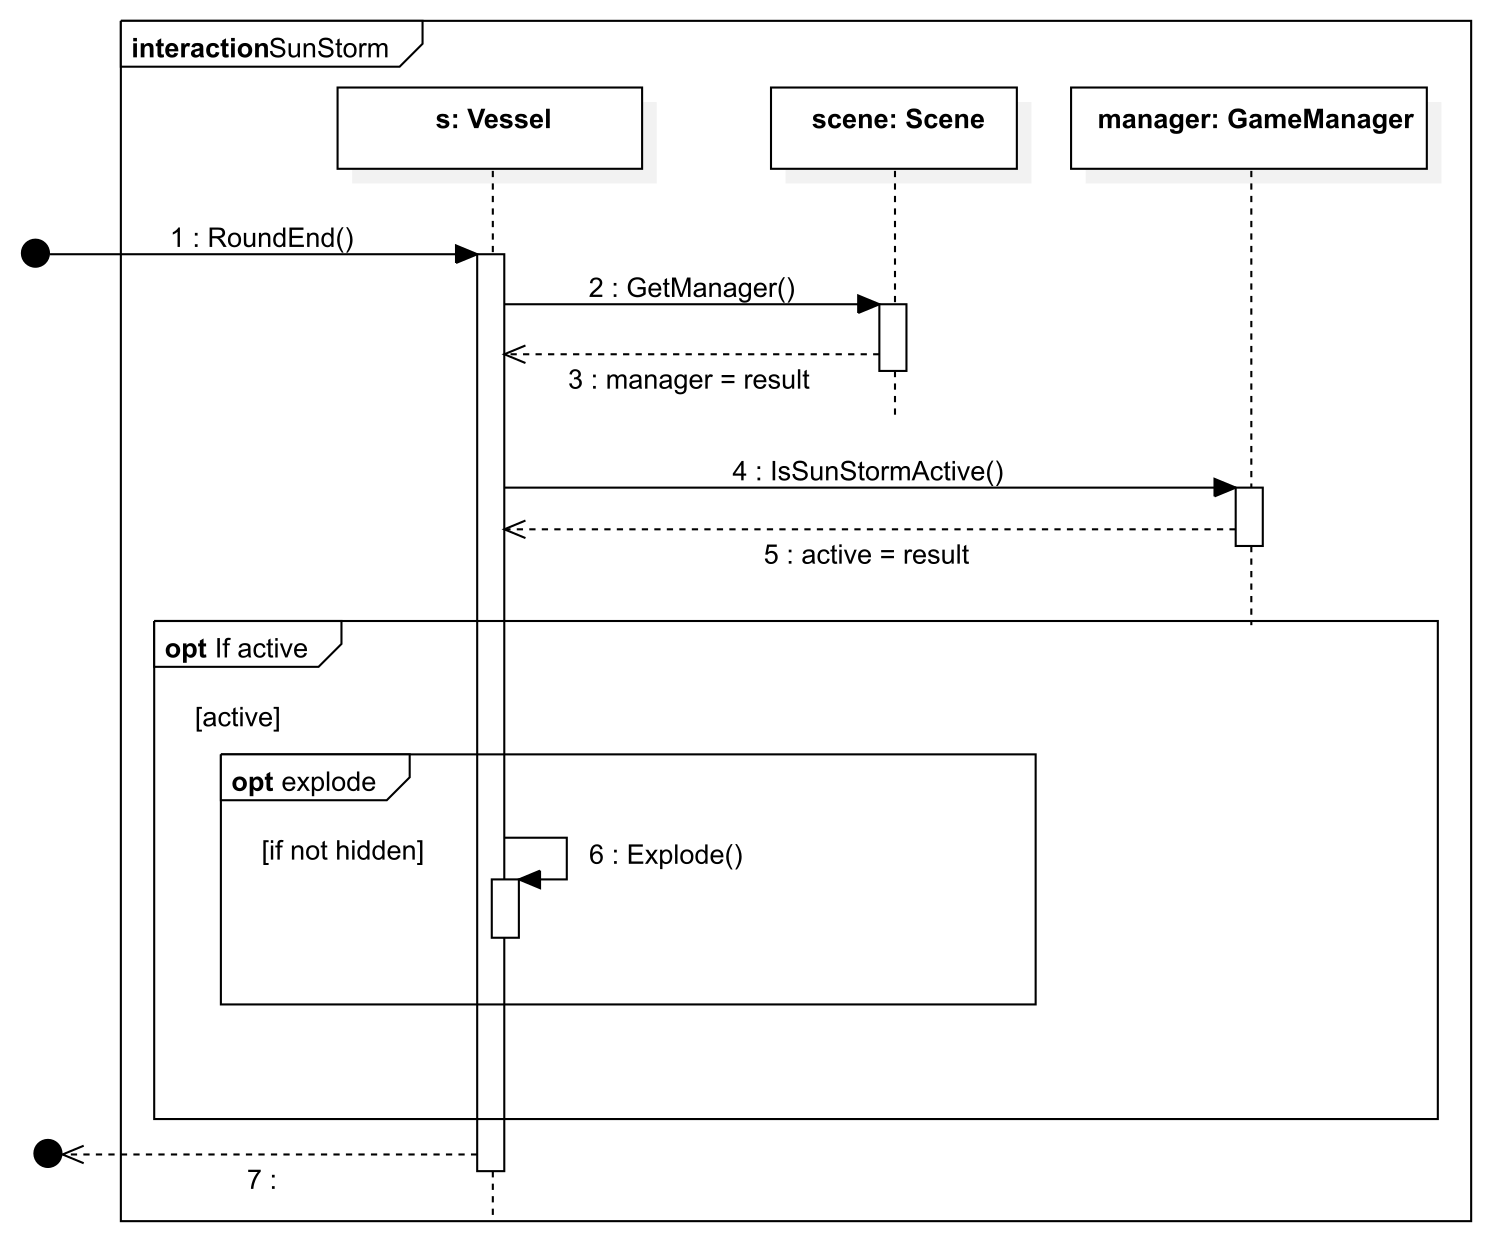
\includegraphics[width=1\textwidth]{docs/3_Project/svg/Design Model!Sun storm!Sun Storm!SunStorm_18.png} 
\caption{...} 
\end{figure} 

\begin{figure}[H] 
\centering 
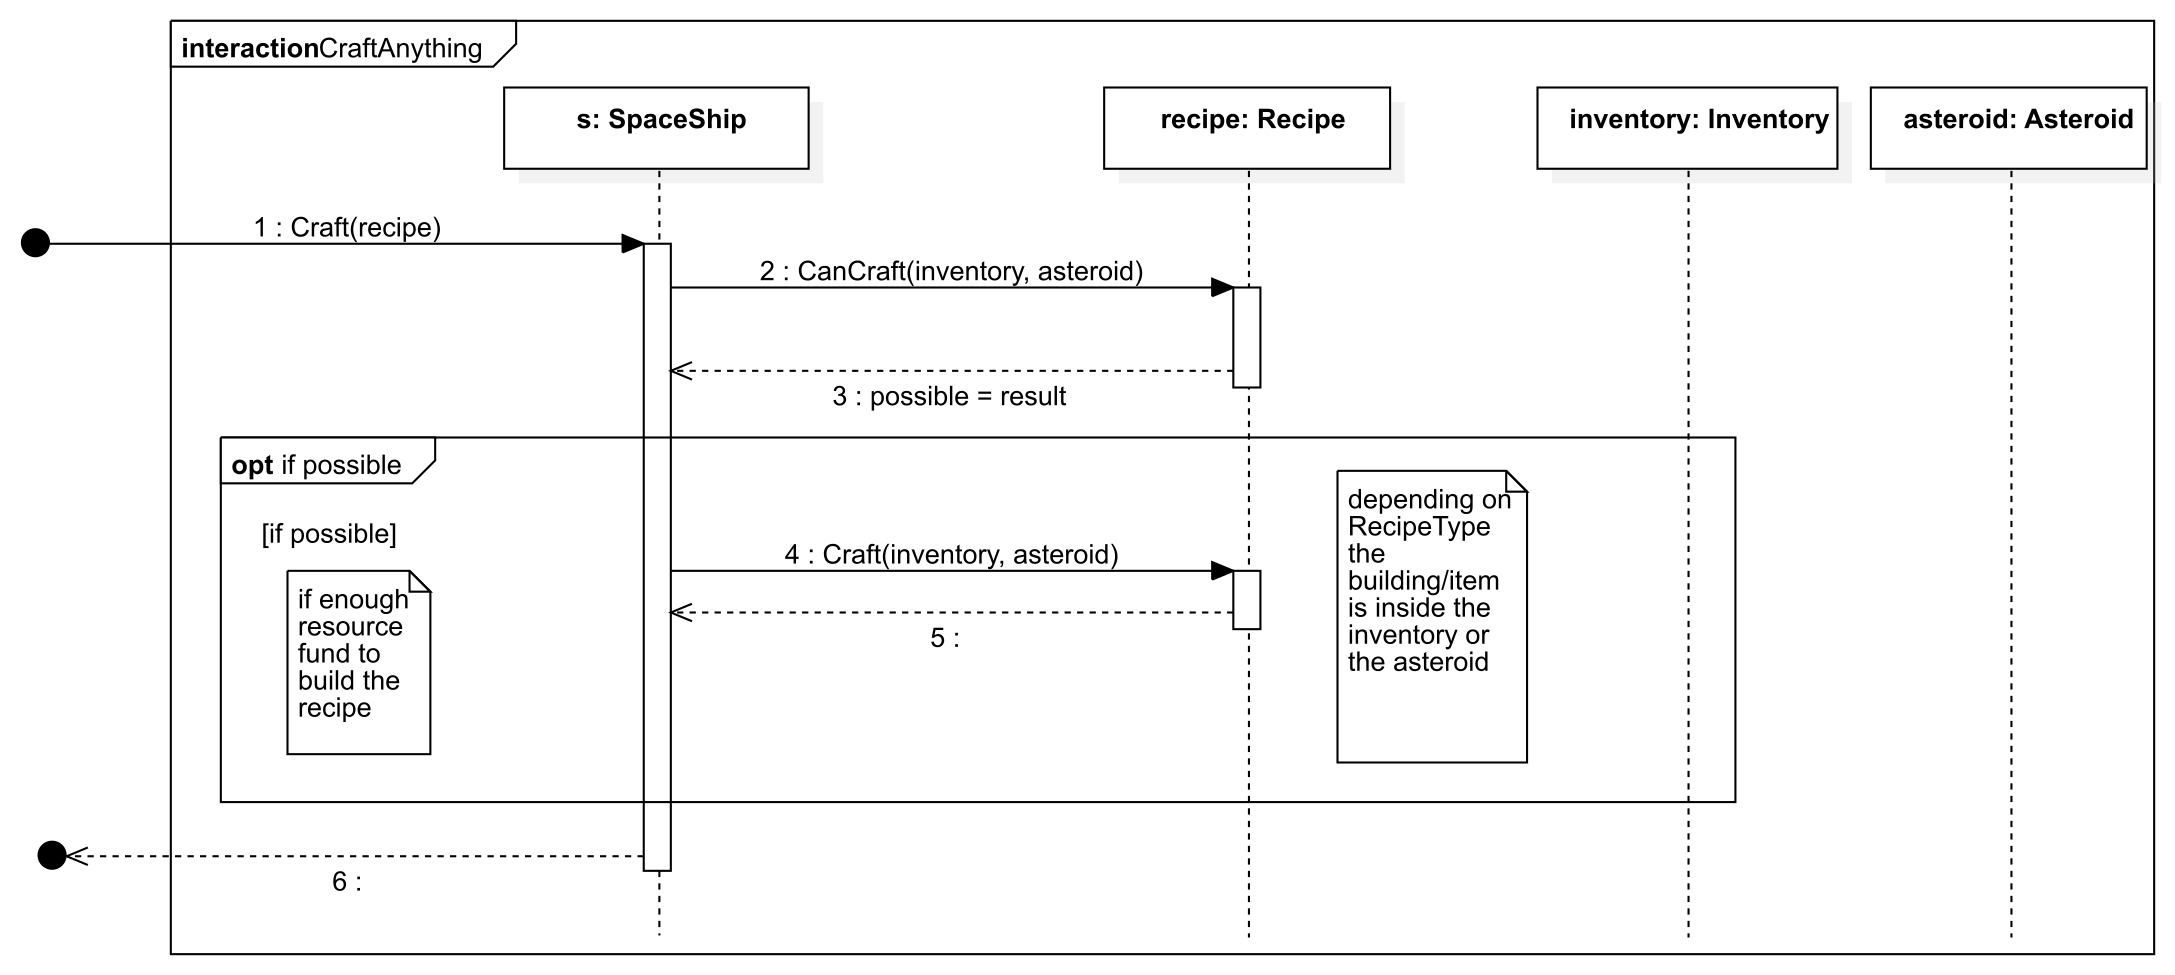
\includegraphics[width=1\textwidth]{docs/3_Project/svg/Design Model!Crafting!Craft!CraftAnything_19.png} 
\caption{A telepes szeretne létrehozni valamit a kibányászott nyerssanyagokkal.} 
\end{figure} 

\begin{figure}[H] 
\centering 
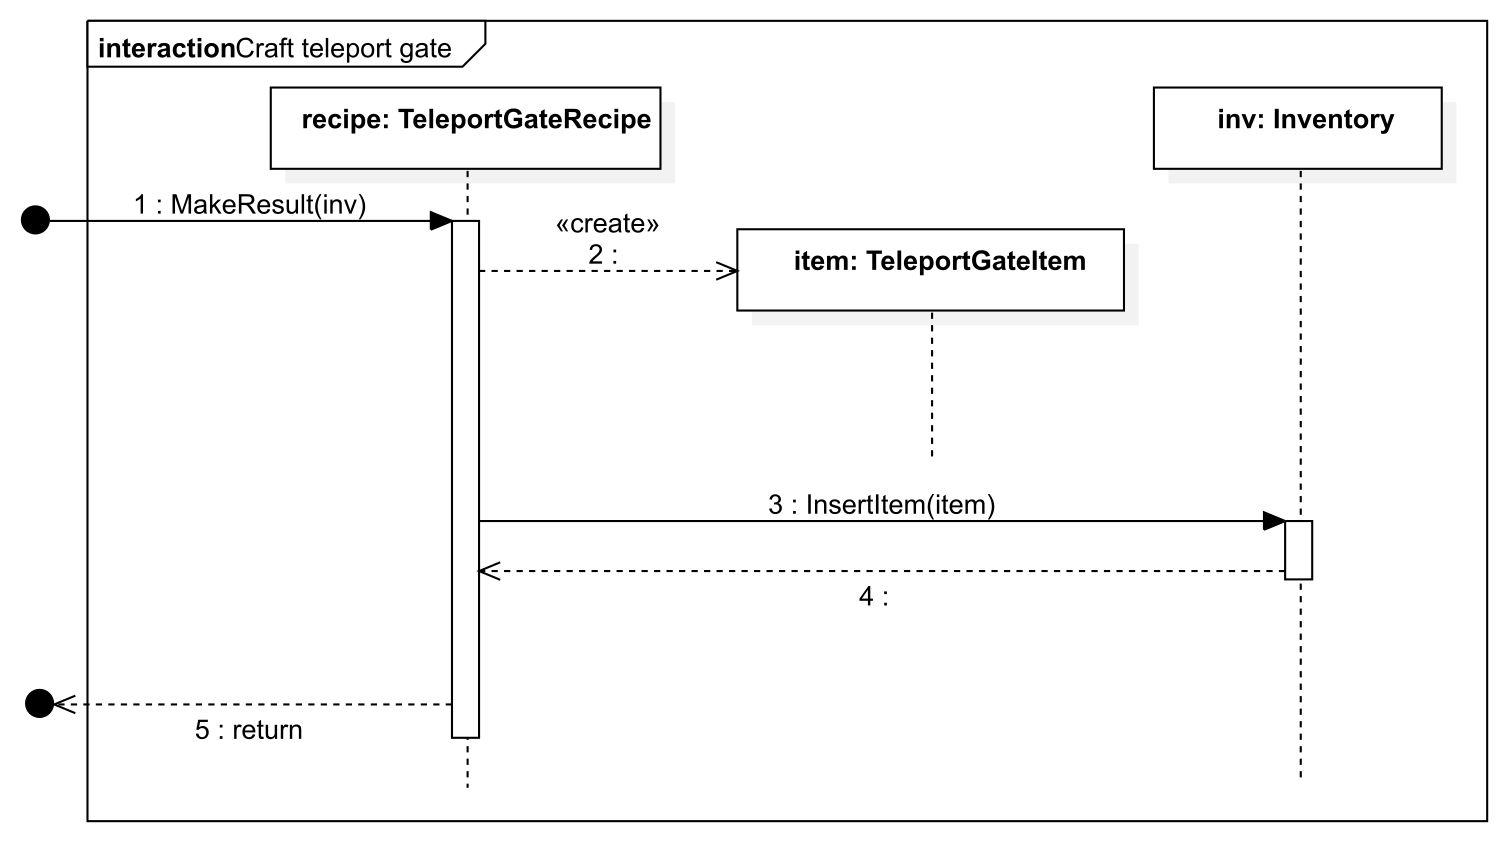
\includegraphics[width=1\textwidth]{docs/3_Project/svg/Design Model!Crafting!Craft teleport gate!Craft teleport gate_20.png} 
\caption{Hogyan jön létre egy új teleportkapu-pár.} 
\end{figure} 

\begin{figure}[H] 
\centering 
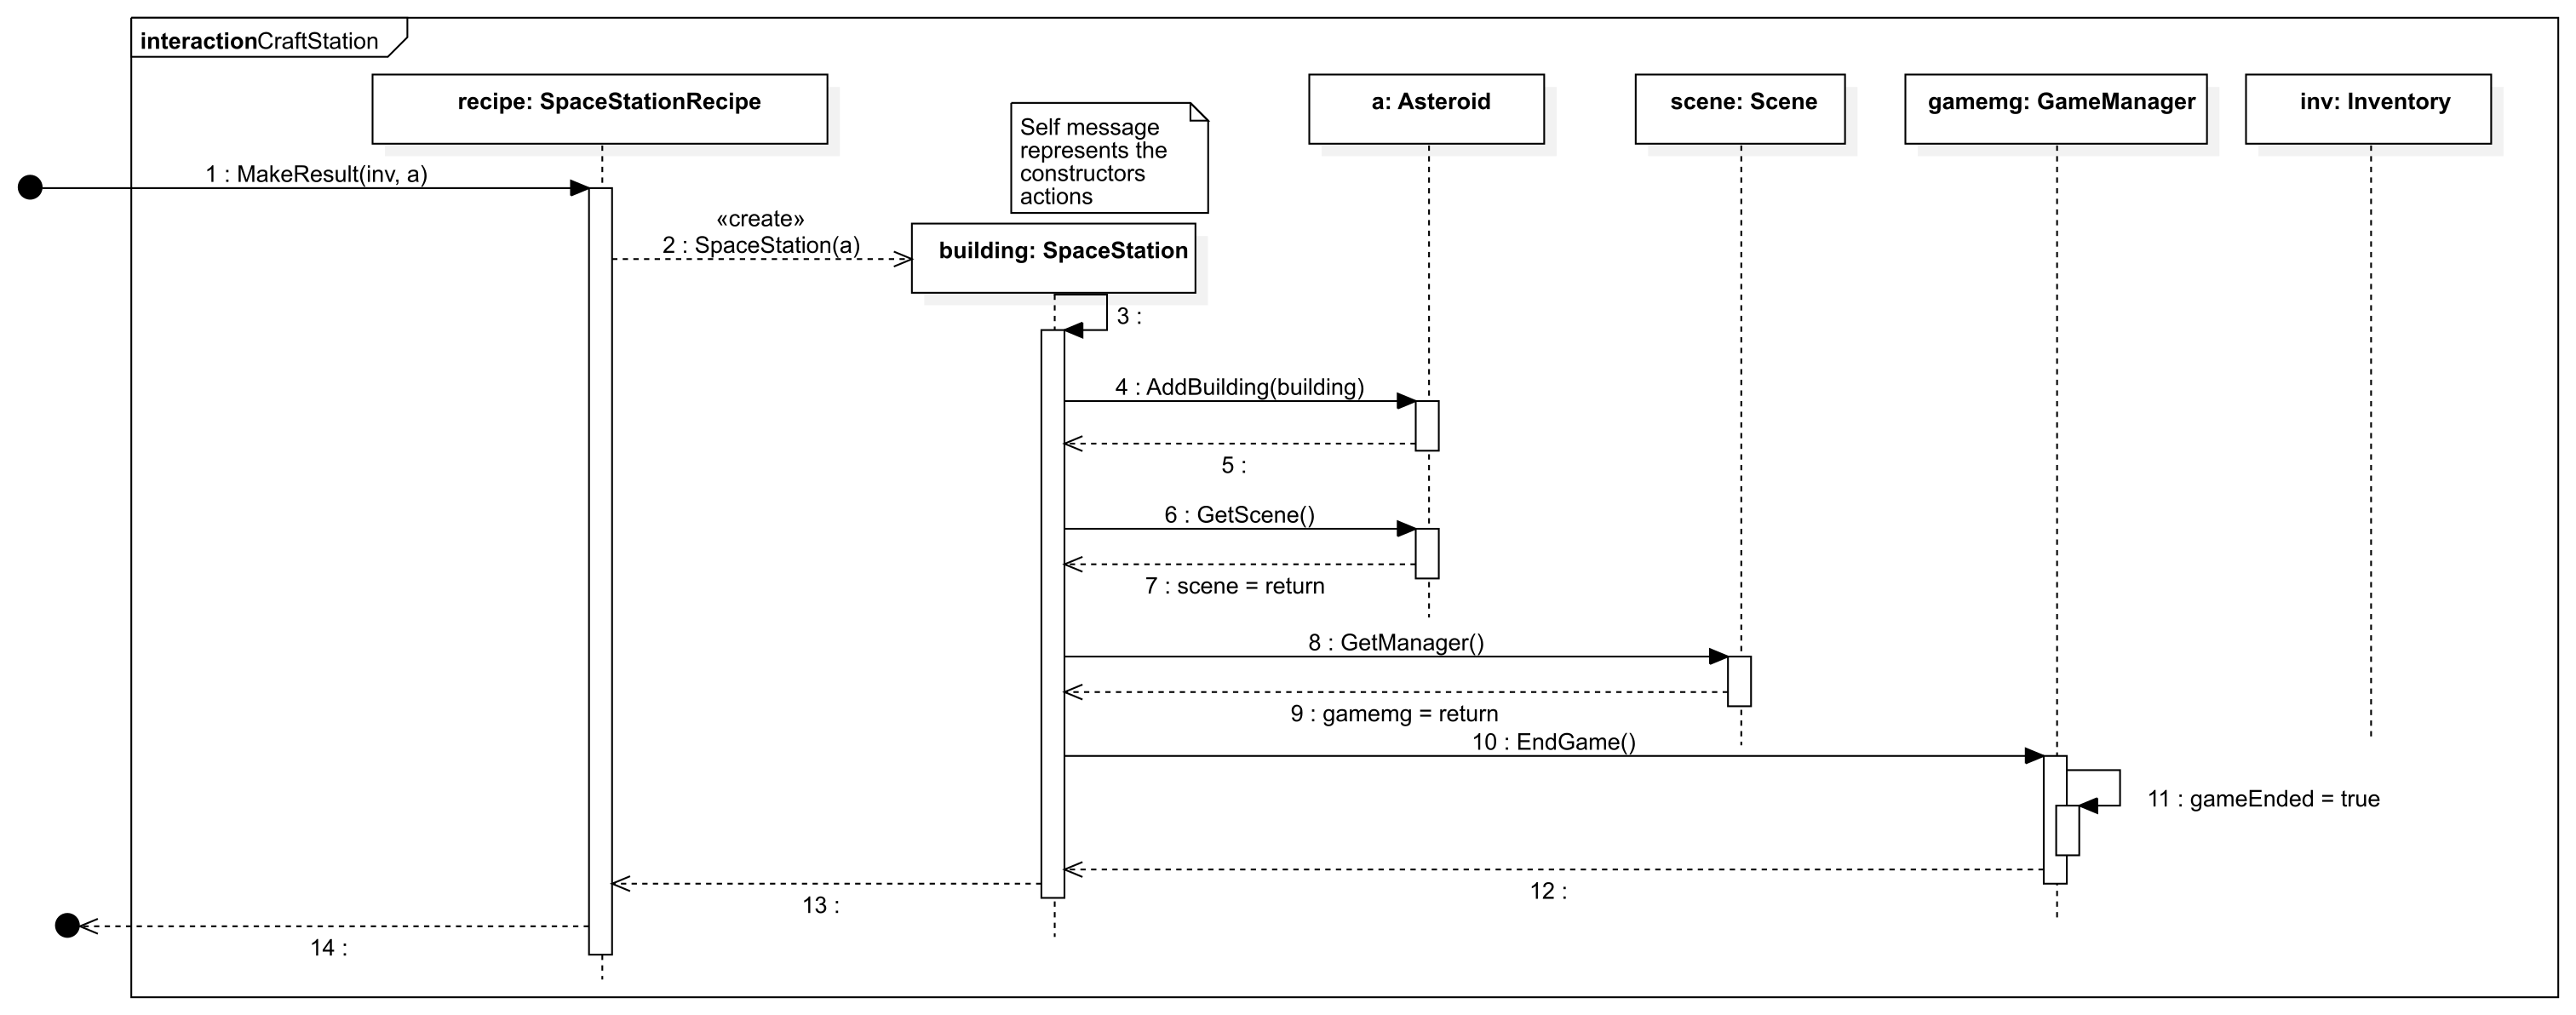
\includegraphics[width=1\textwidth]{docs/3_Project/svg/Design Model!Crafting!CraftStation!CraftStation_21.png} 
\caption{Ha a telepesek megcsinálnak egy bázist, akkor megnyerik a játékot.} 
\end{figure} 

\begin{figure}[H] 
\centering 
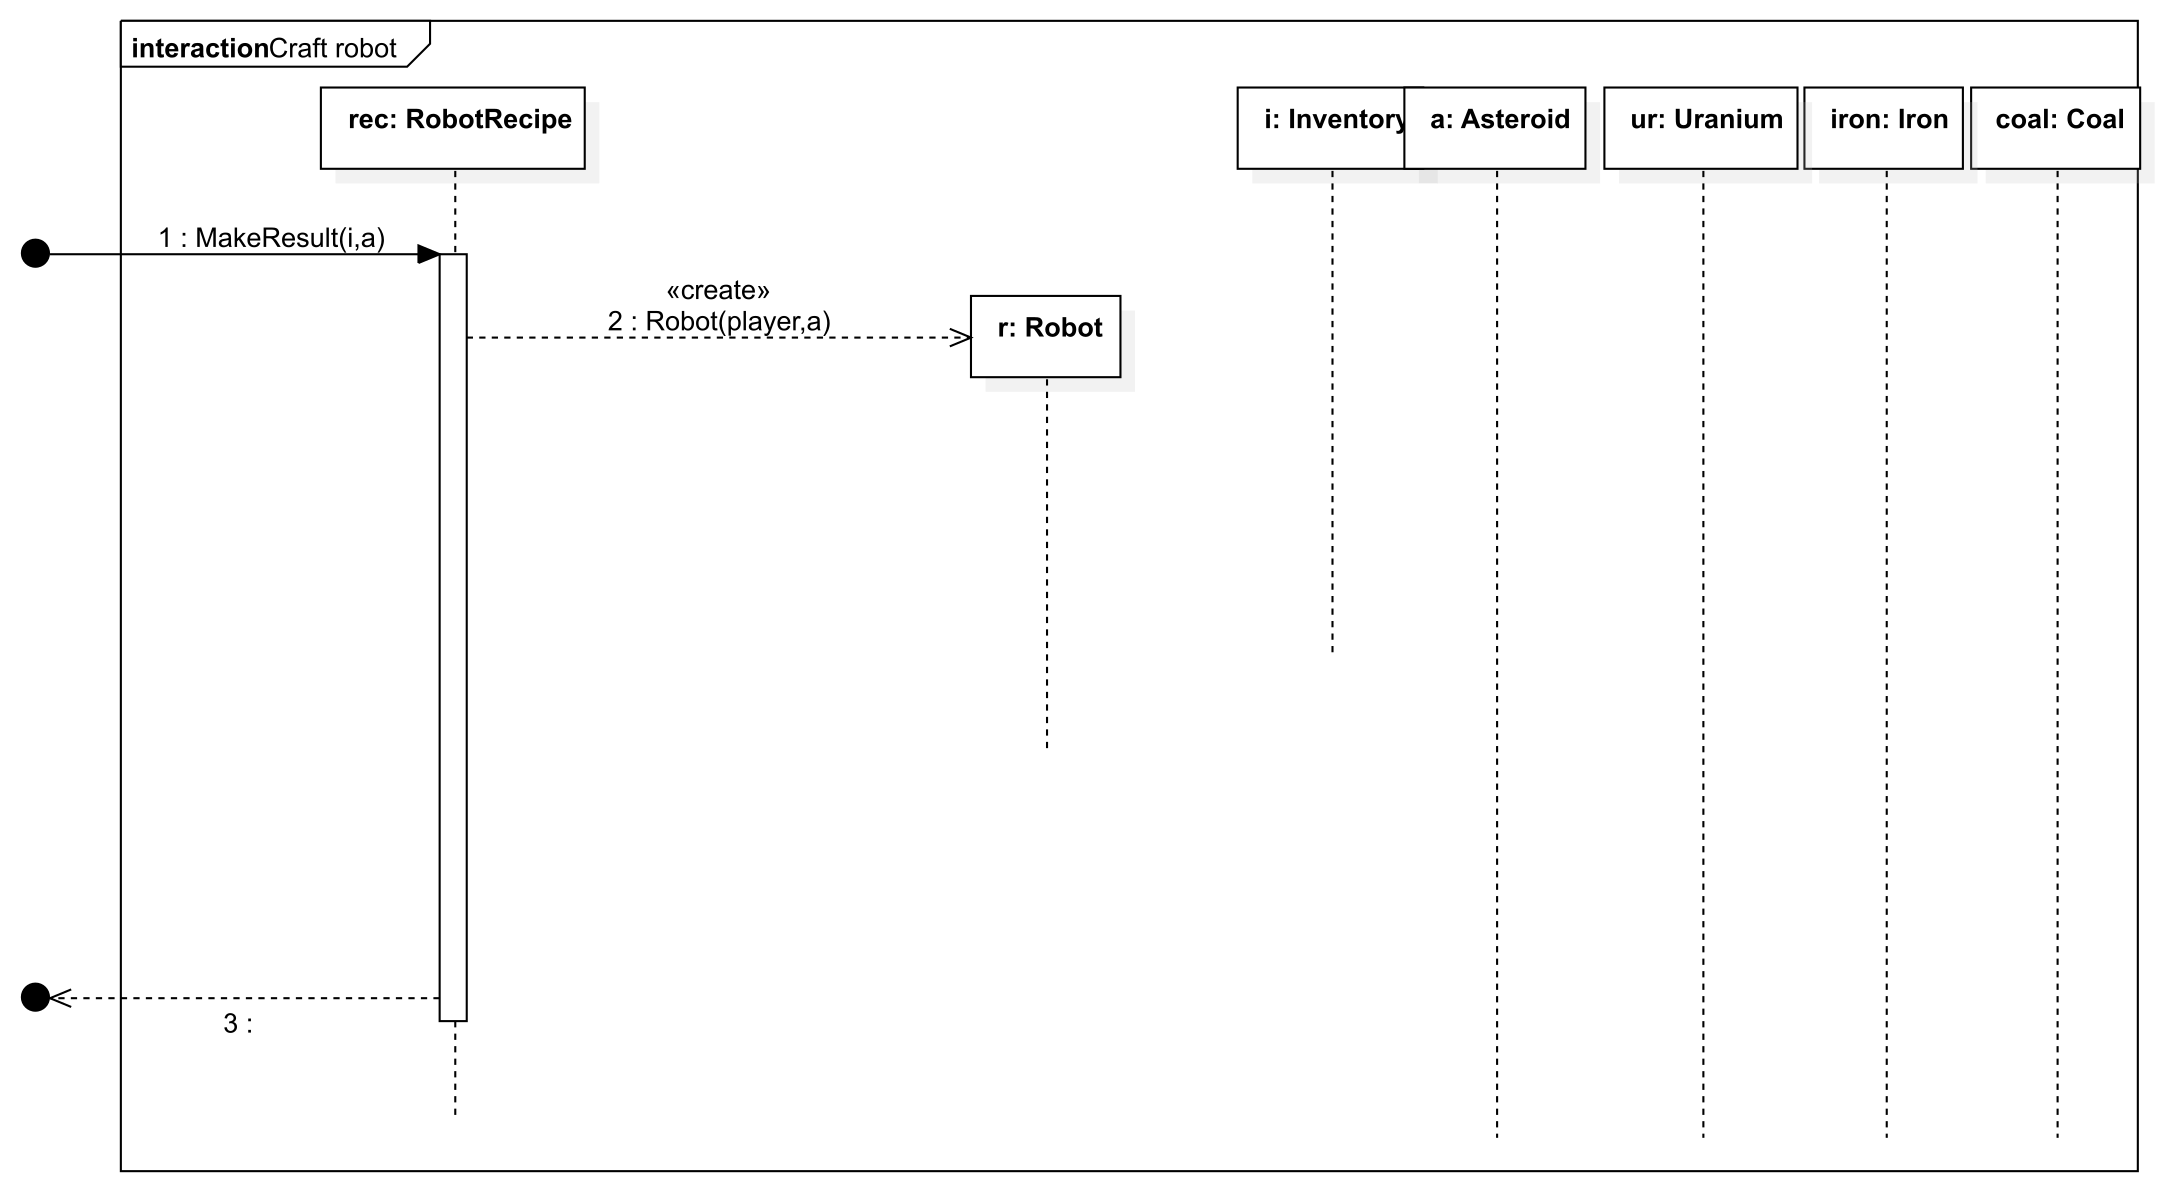
\includegraphics[width=1\textwidth]{docs/3_Project/svg/Design Model!Crafting!Craft robot!Craft robot_22.png} 
\caption{A robot létrehozása azonnal lehelyezi a robotot.} 
\end{figure} 

\begin{figure}[H] 
\centering 
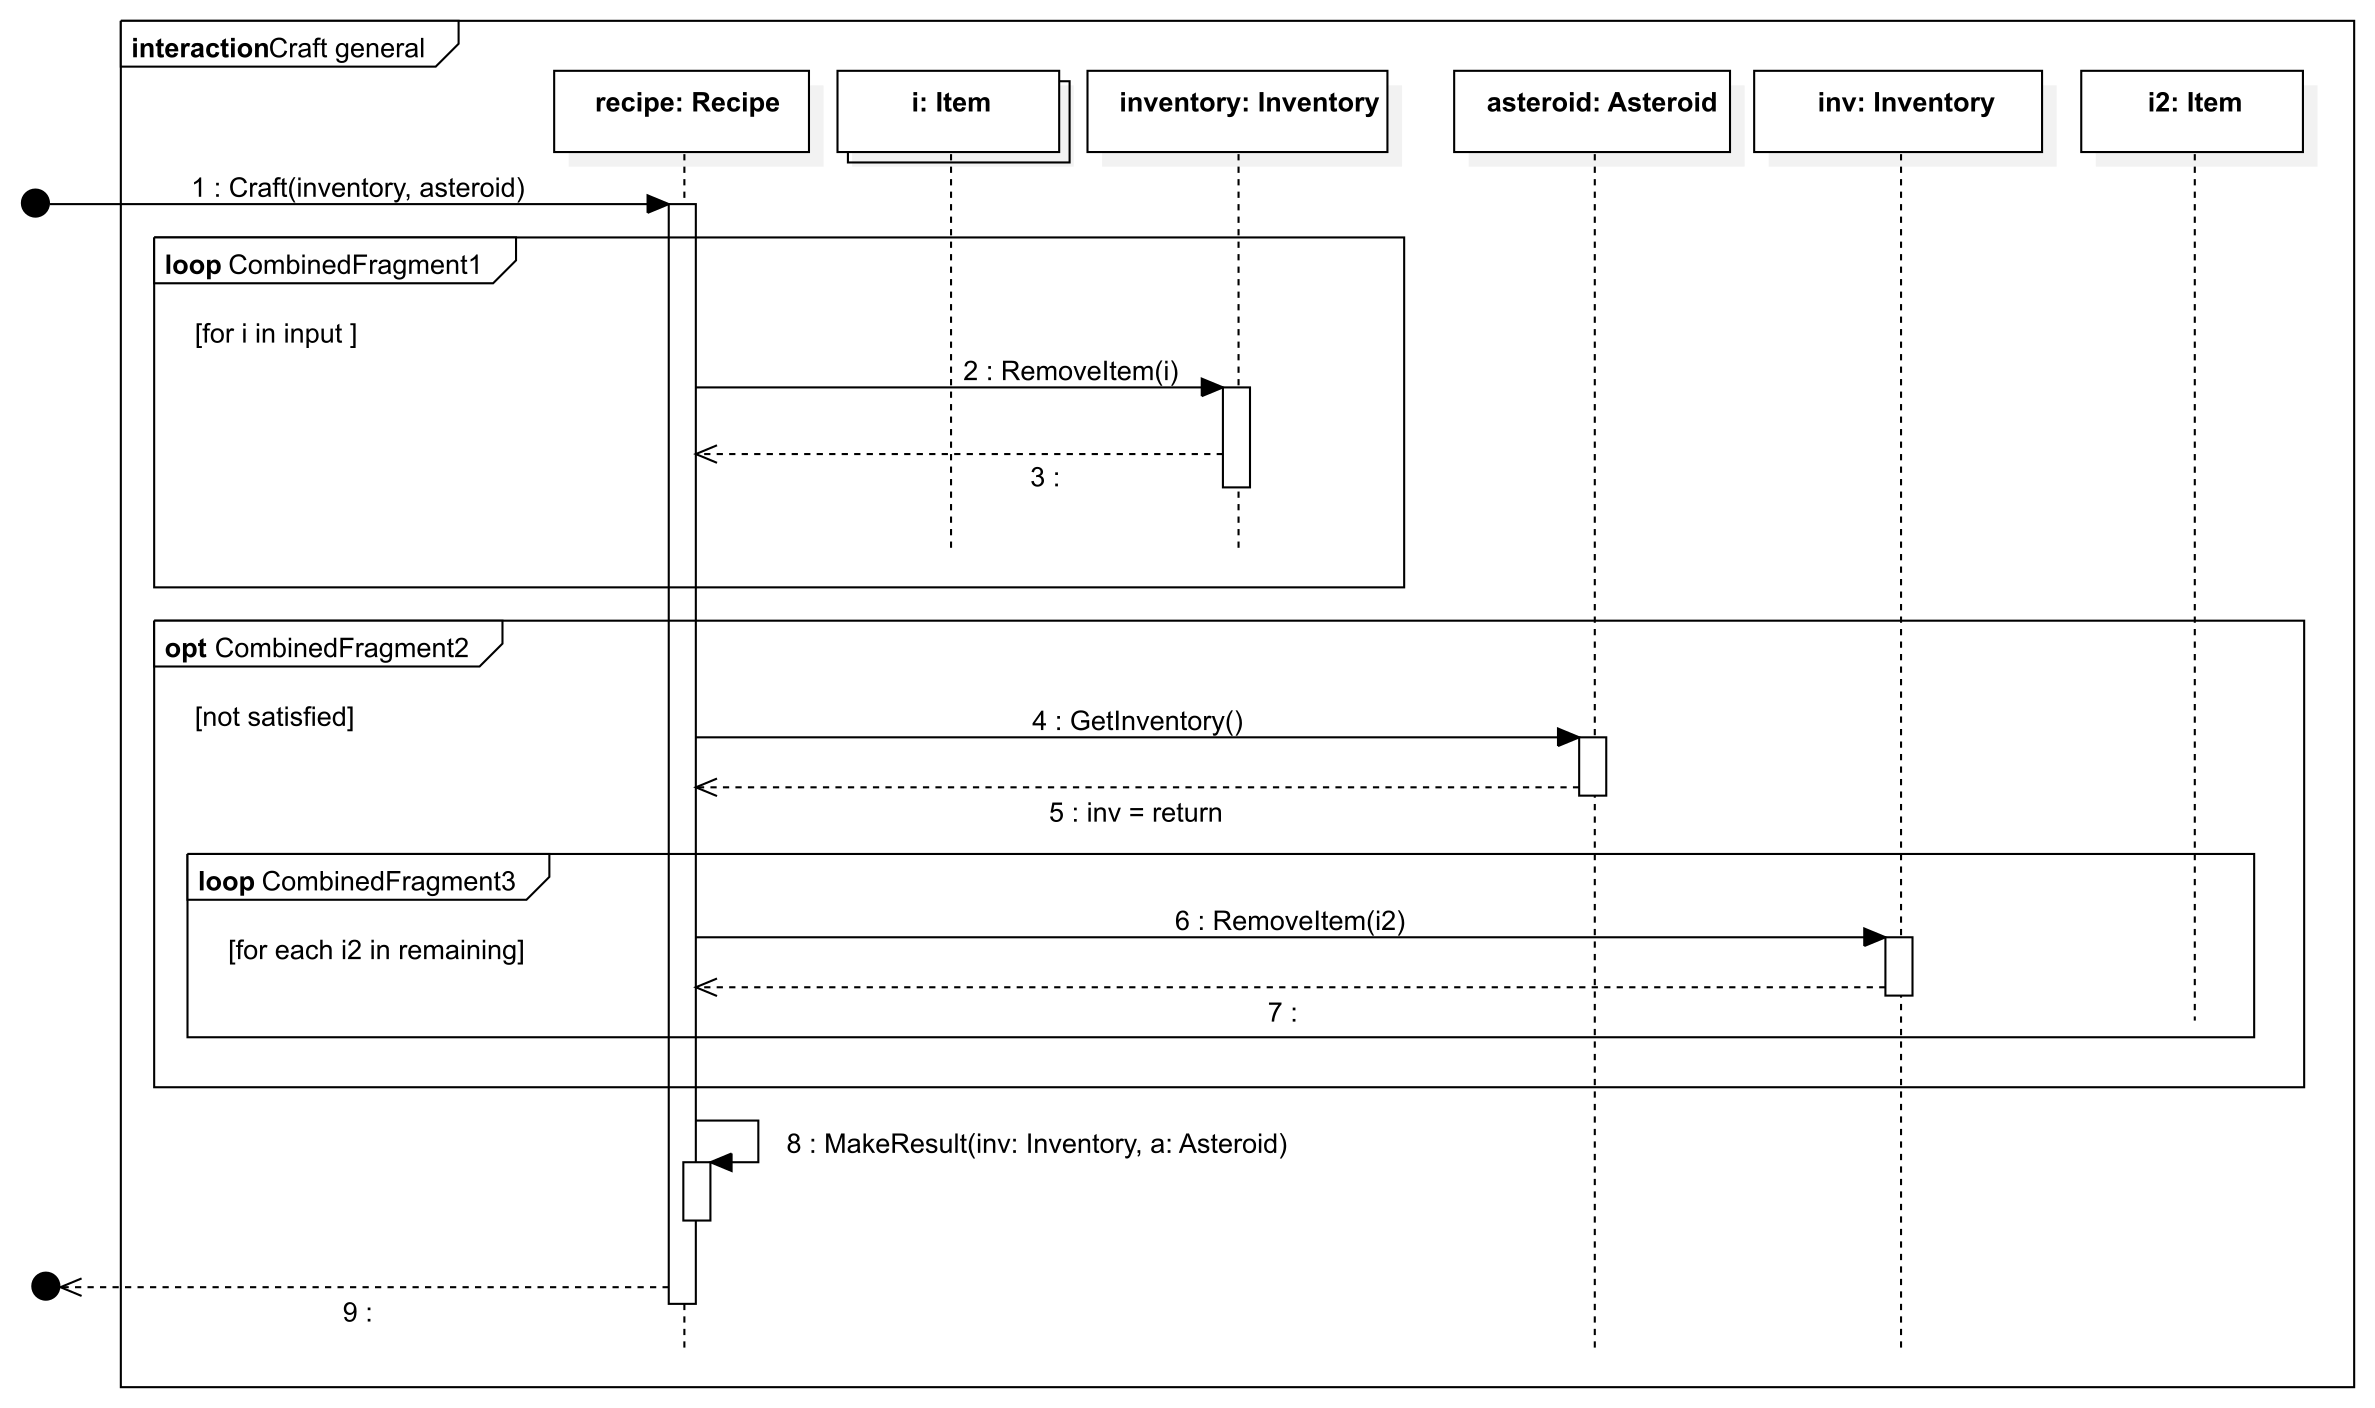
\includegraphics[width=1\textwidth]{docs/3_Project/svg/Design Model!Crafting!Craft general!Craft general_23.png} 
\caption{A recept levonja a nyersanyagokat, ha el tudjuk készíteni a tárgyat.} 
\end{figure} 

\begin{figure}[H] 
\centering 
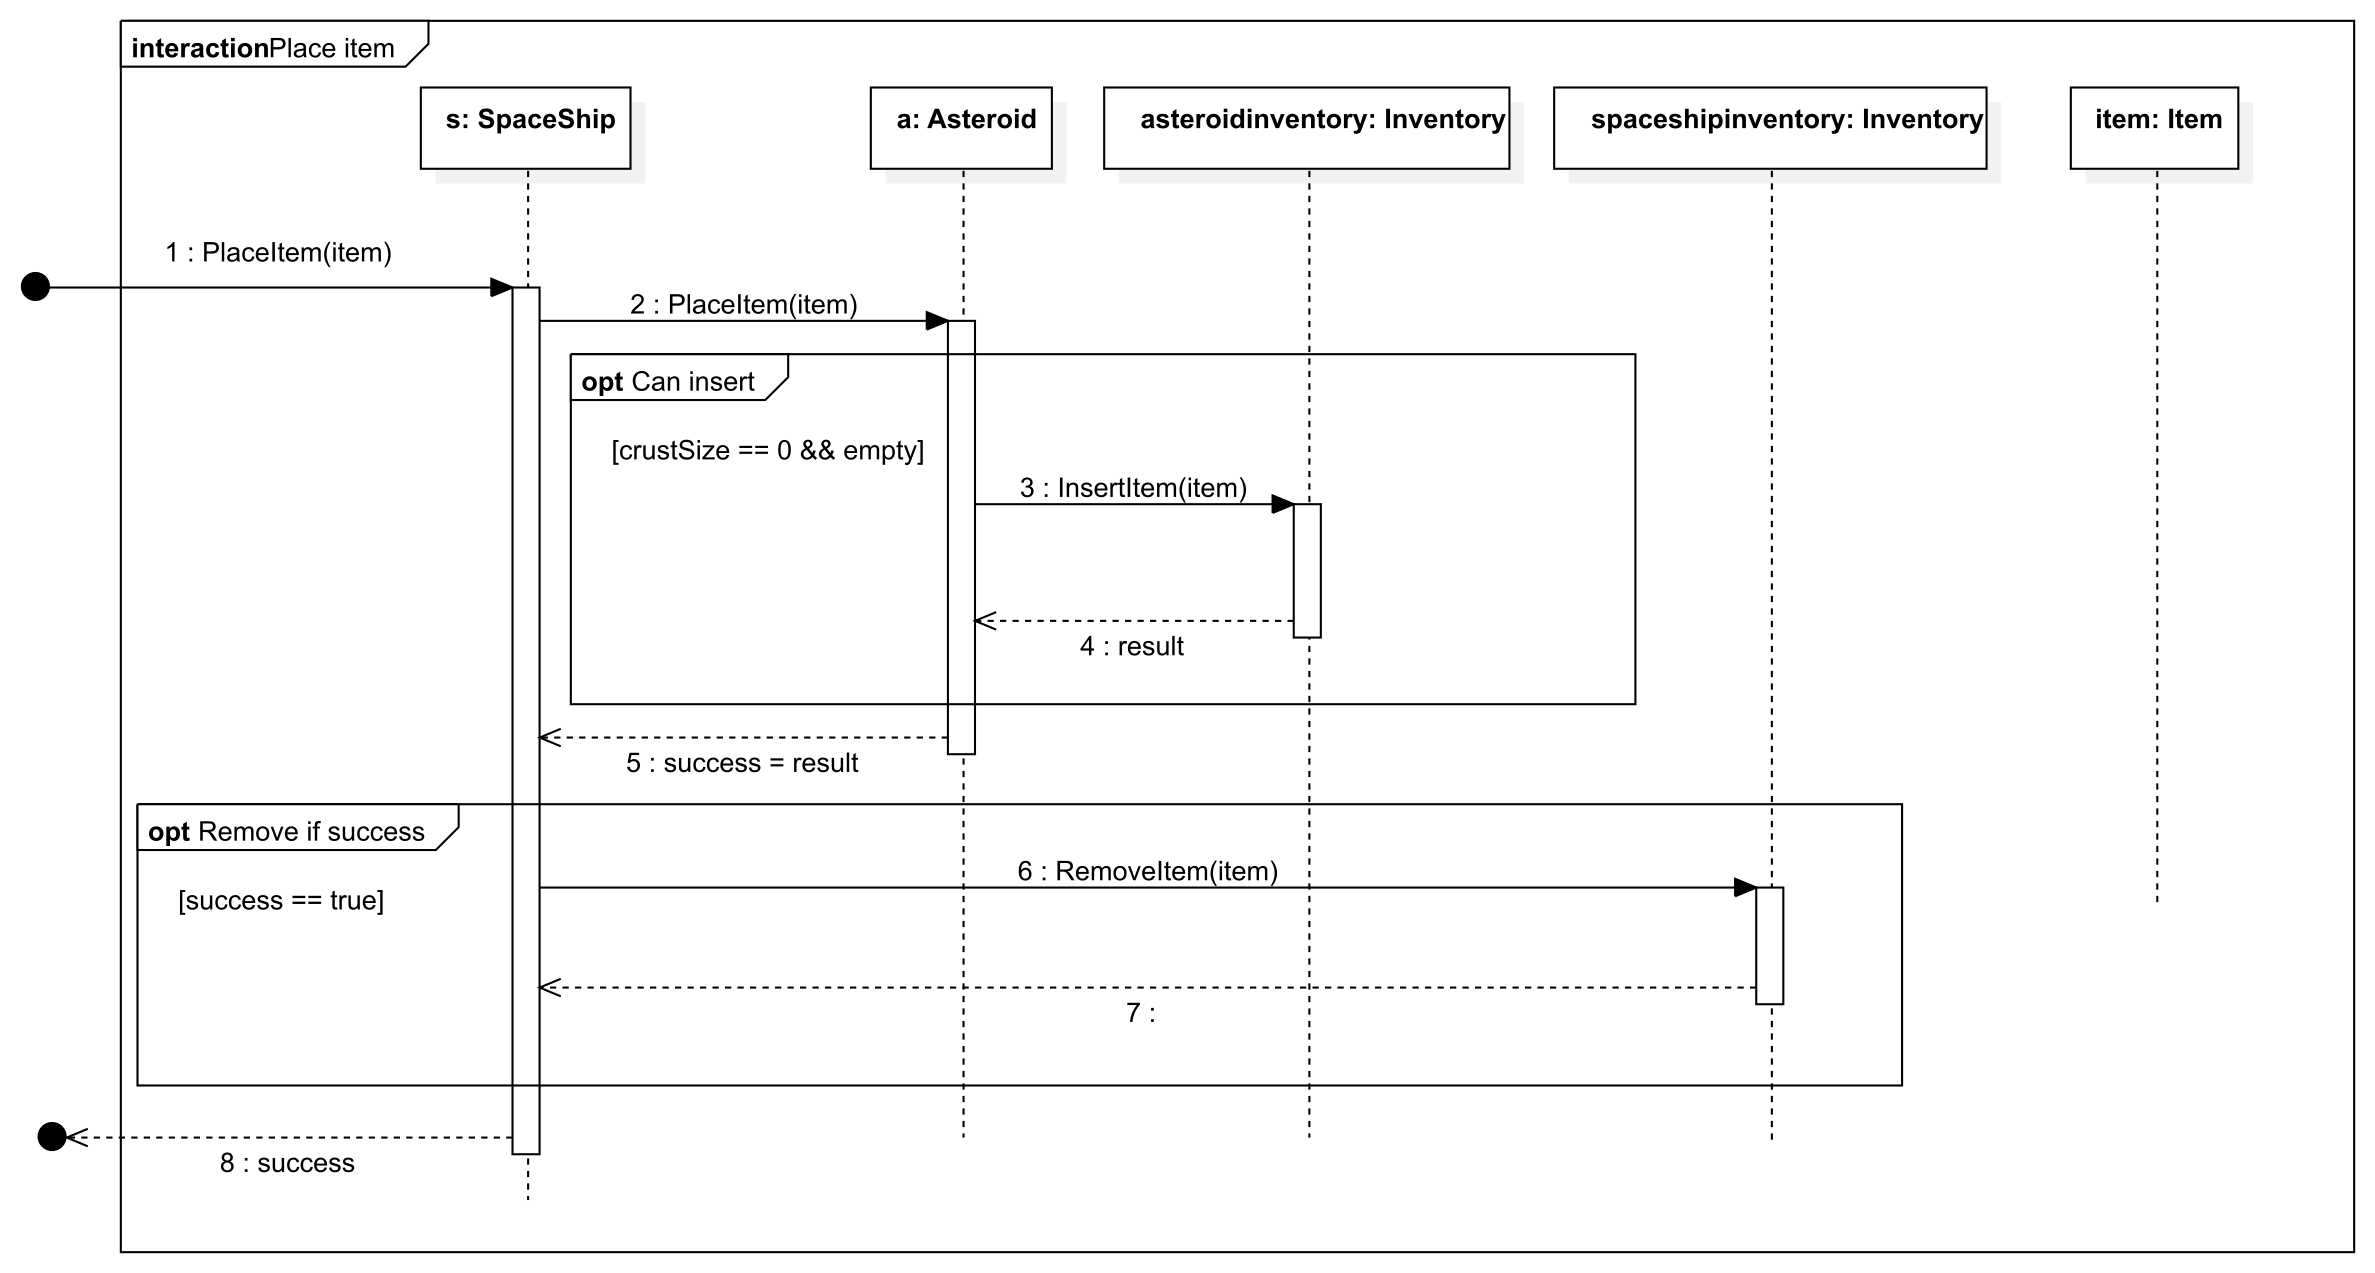
\includegraphics[width=1\textwidth]{docs/3_Project/svg/Design Model!Place resource in inventory!successful placement!Place item_24.png} 
\caption{Lehelyezünk egy tárgyat az átfúrt kérgű, üreges aszteroidába.} 
\end{figure} 

\begin{figure}[H] 
\centering 
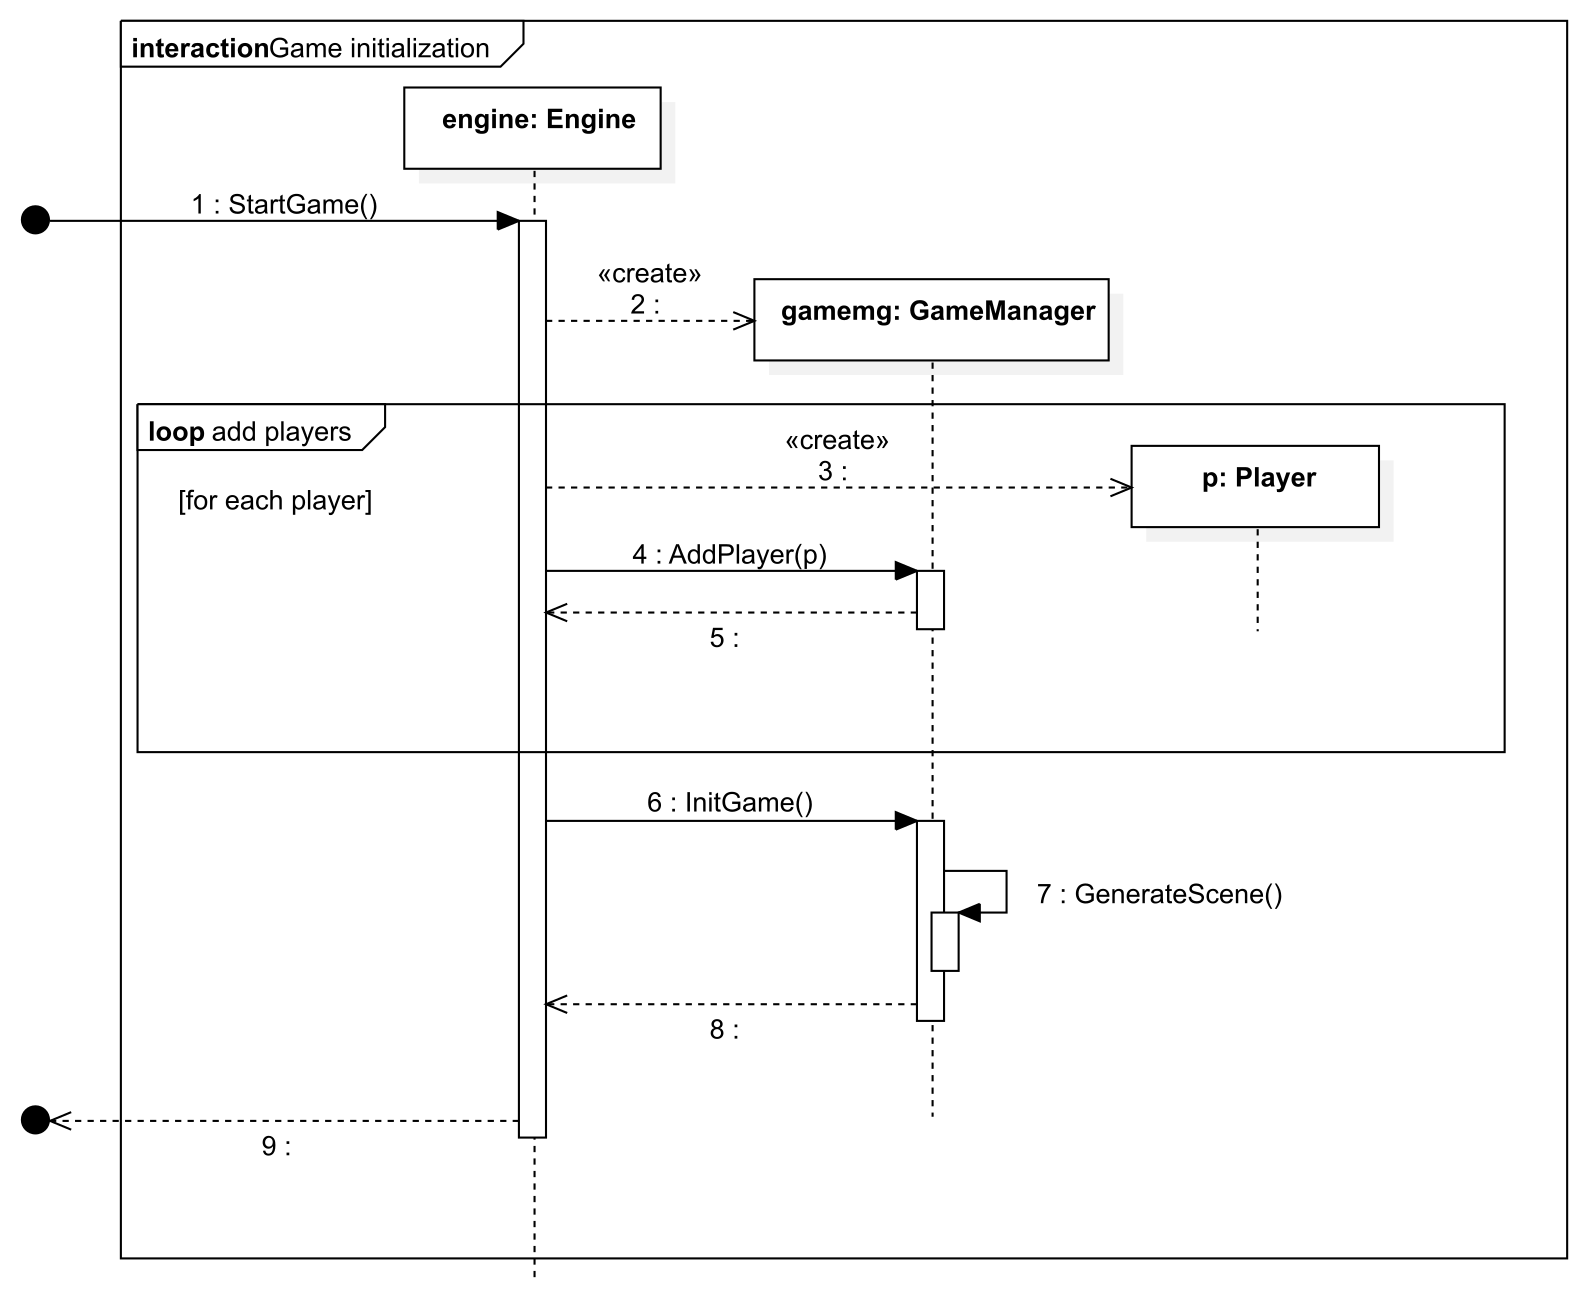
\includegraphics[width=1\textwidth]{docs/3_Project/svg/Design Model!Game Init!Game initialization!Game initialization_25.png} 
\caption{A játék indítása hogyan megy végbe.} 
\end{figure} 

\begin{figure}[H] 
\centering 
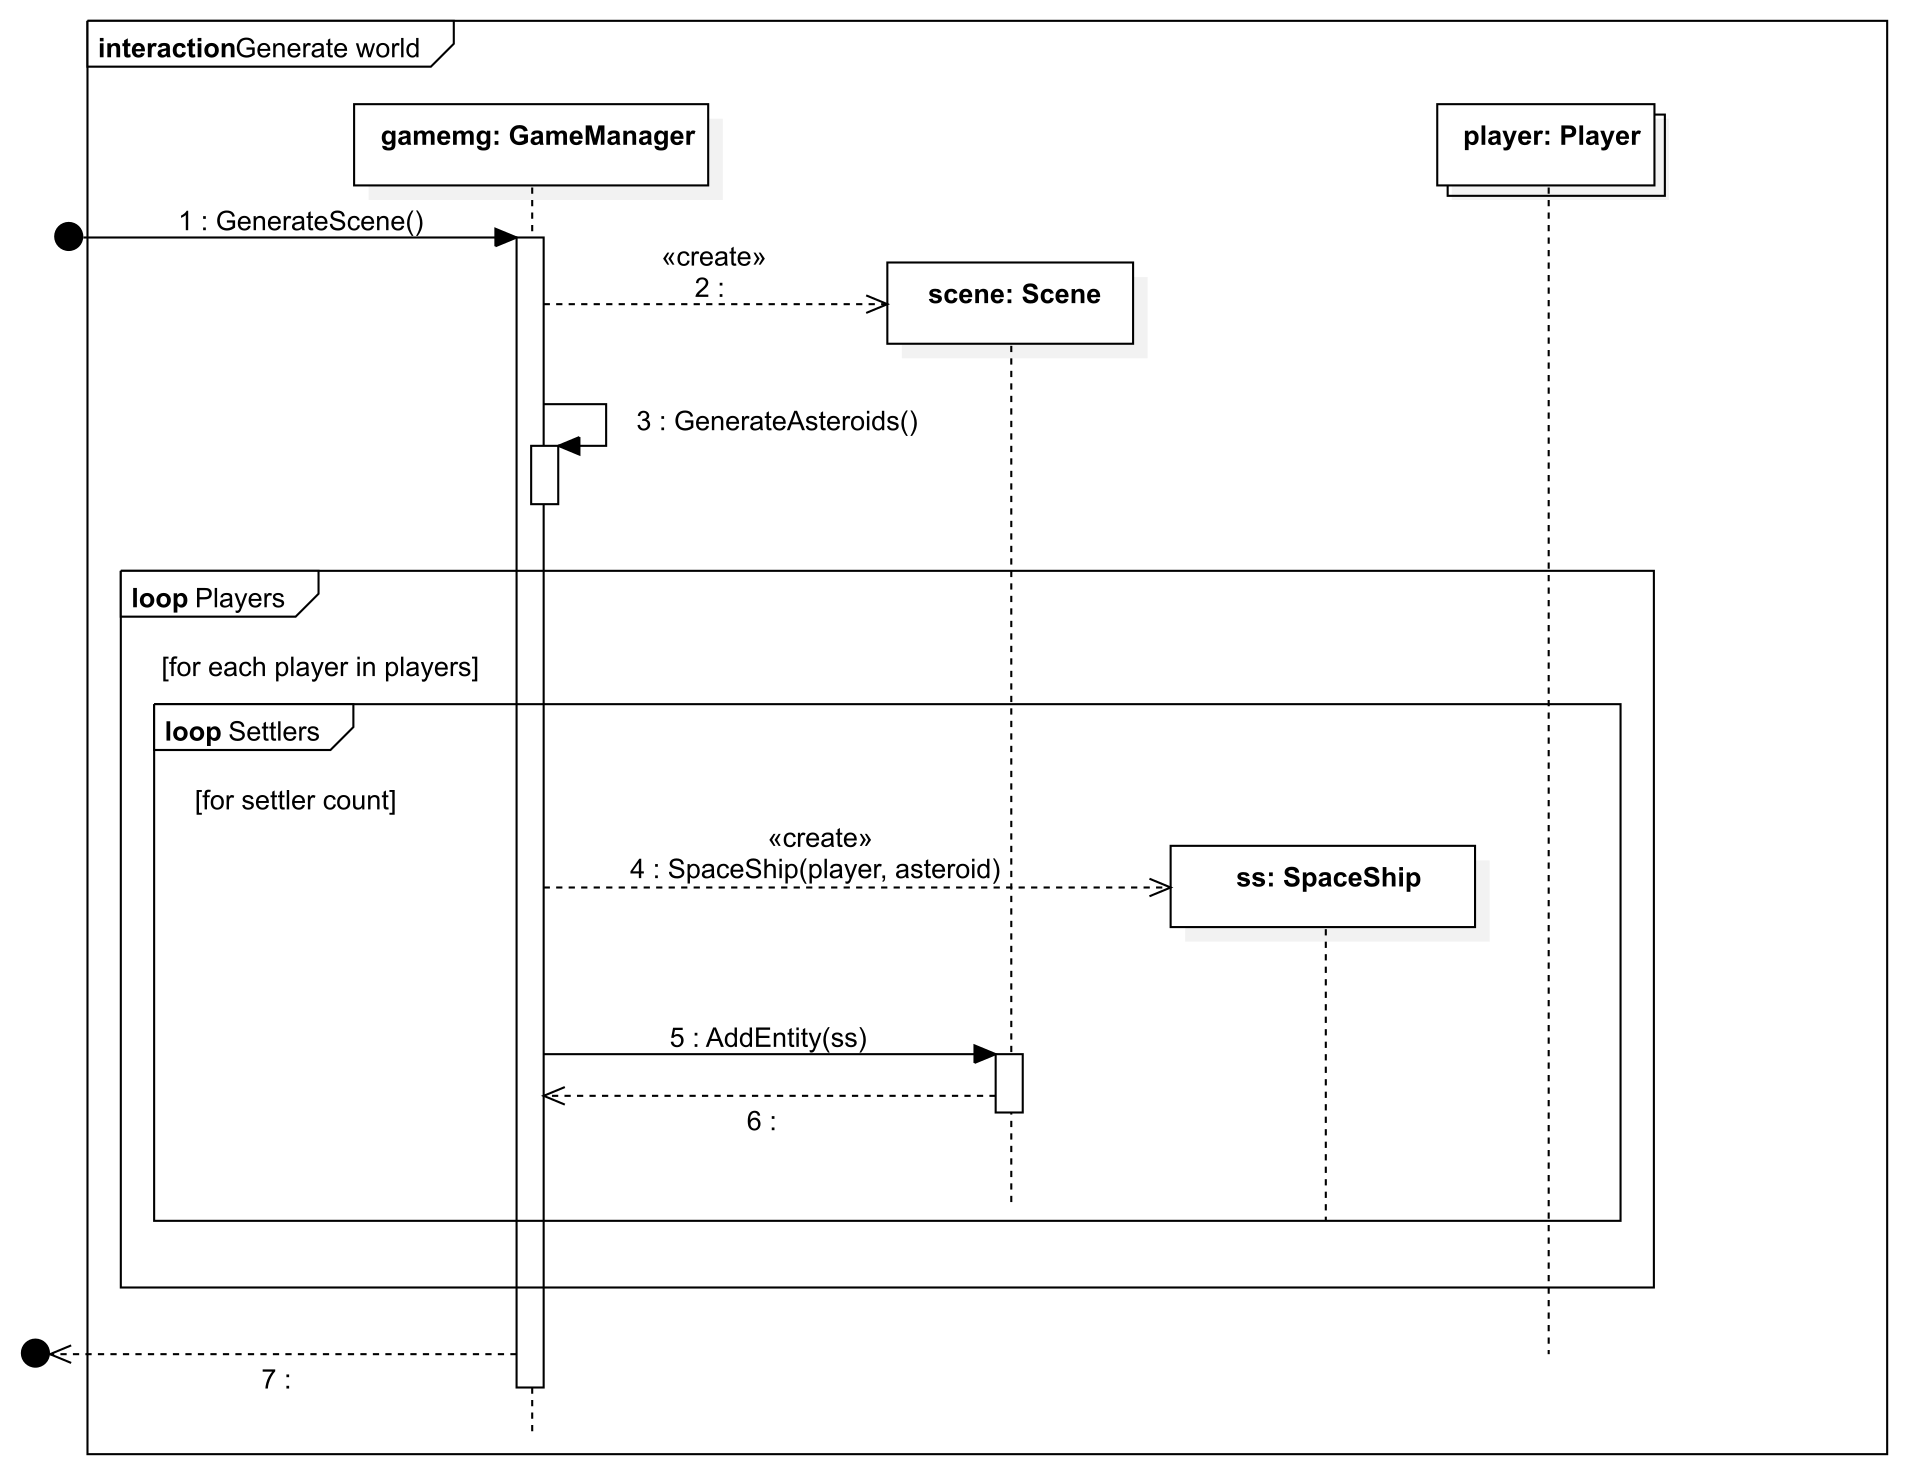
\includegraphics[width=1\textwidth]{docs/3_Project/svg/Design Model!Game Init!Generate world!Generate world_26.png} 
\caption{A játék indításának az a része, ahol létrejönnek az aszteroidák, és ahol lehelyezzük a telepeseket.} 
\end{figure} 

\begin{figure}[H] 
\centering 
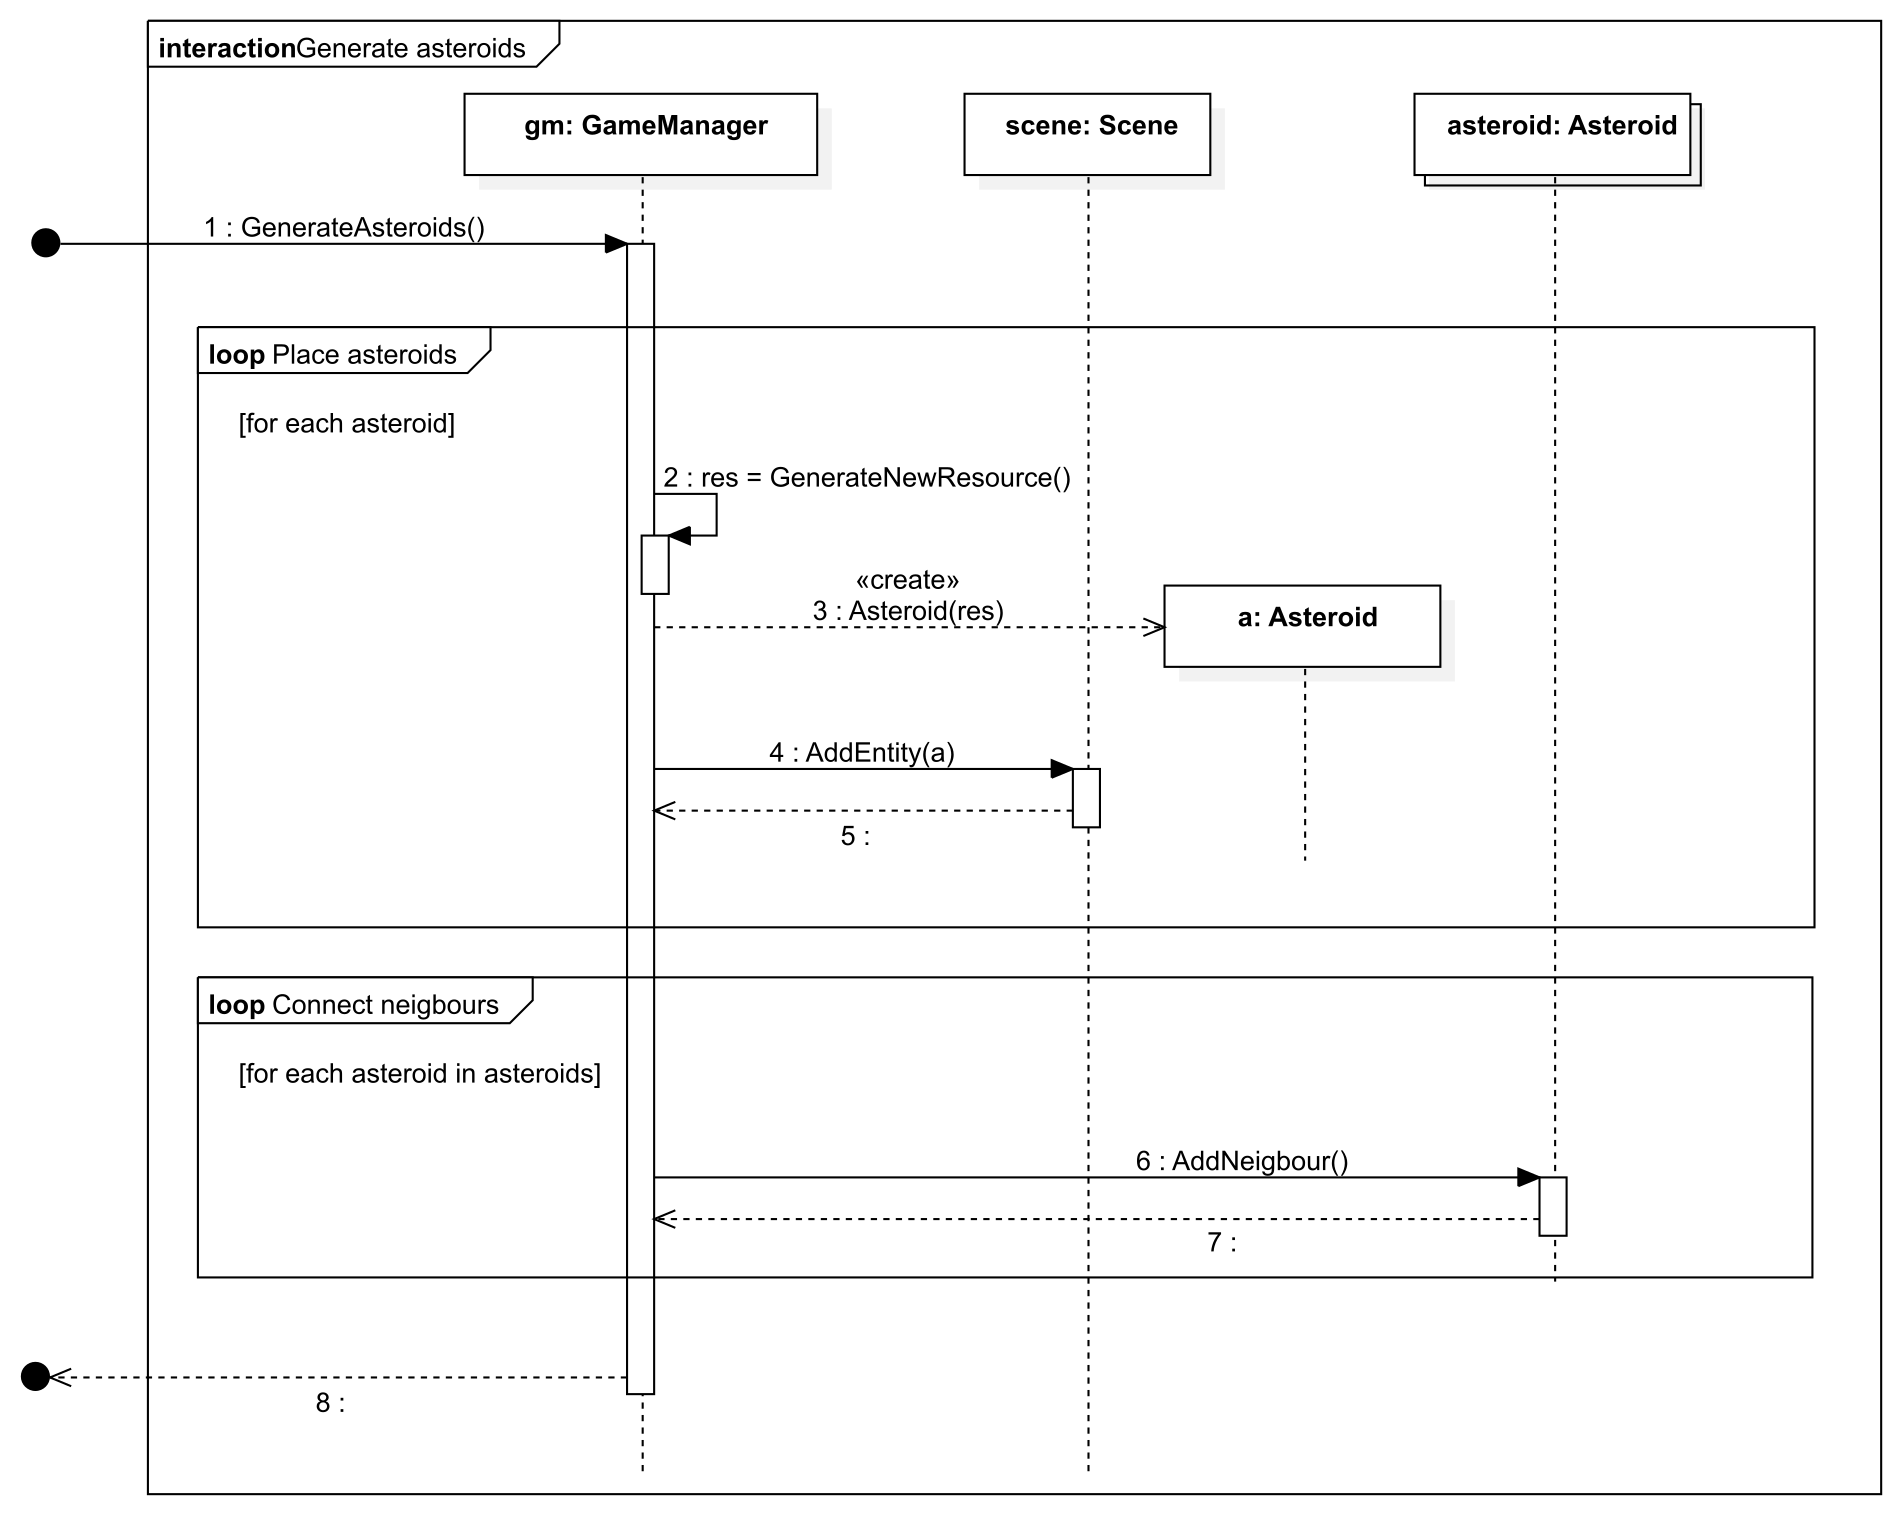
\includegraphics[width=1\textwidth]{docs/3_Project/svg/Design Model!Game Init!Generate asteroids!Generate asteroids_27.png} 
\caption{Az aszteroidák létrehozásának folyamata. Itt telítjük meg őket nyersanyaggal (ha nem üregesek) és itt jön lére a szomszédság is.} 
\end{figure} 

\begin{figure}[H] 
\centering 
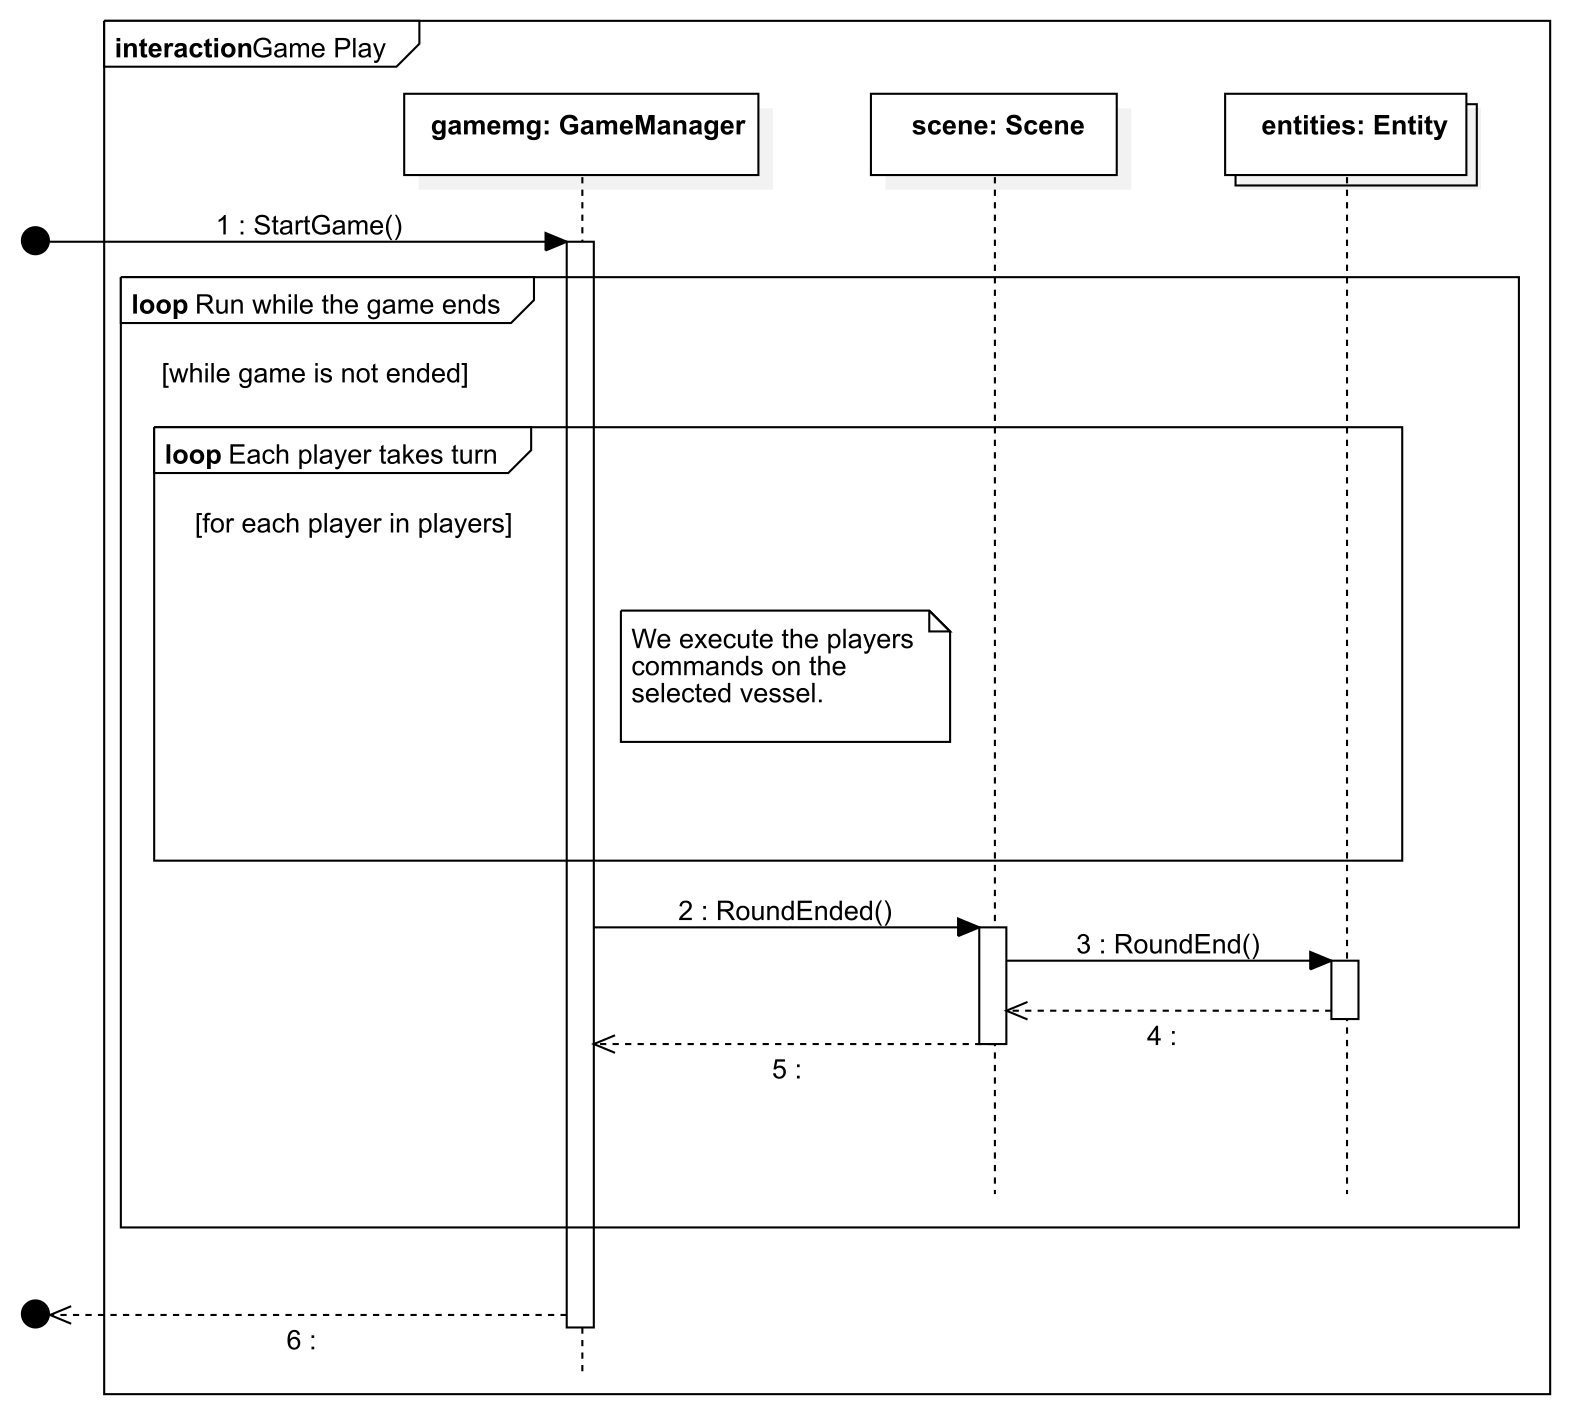
\includegraphics[width=1\textwidth]{docs/3_Project/svg/Design Model!Game play!Game Play!Game Play_28.png} 
\caption{A játék lefutásának felső szintje.} 
\end{figure} 

\begin{figure}[H] 
\centering 
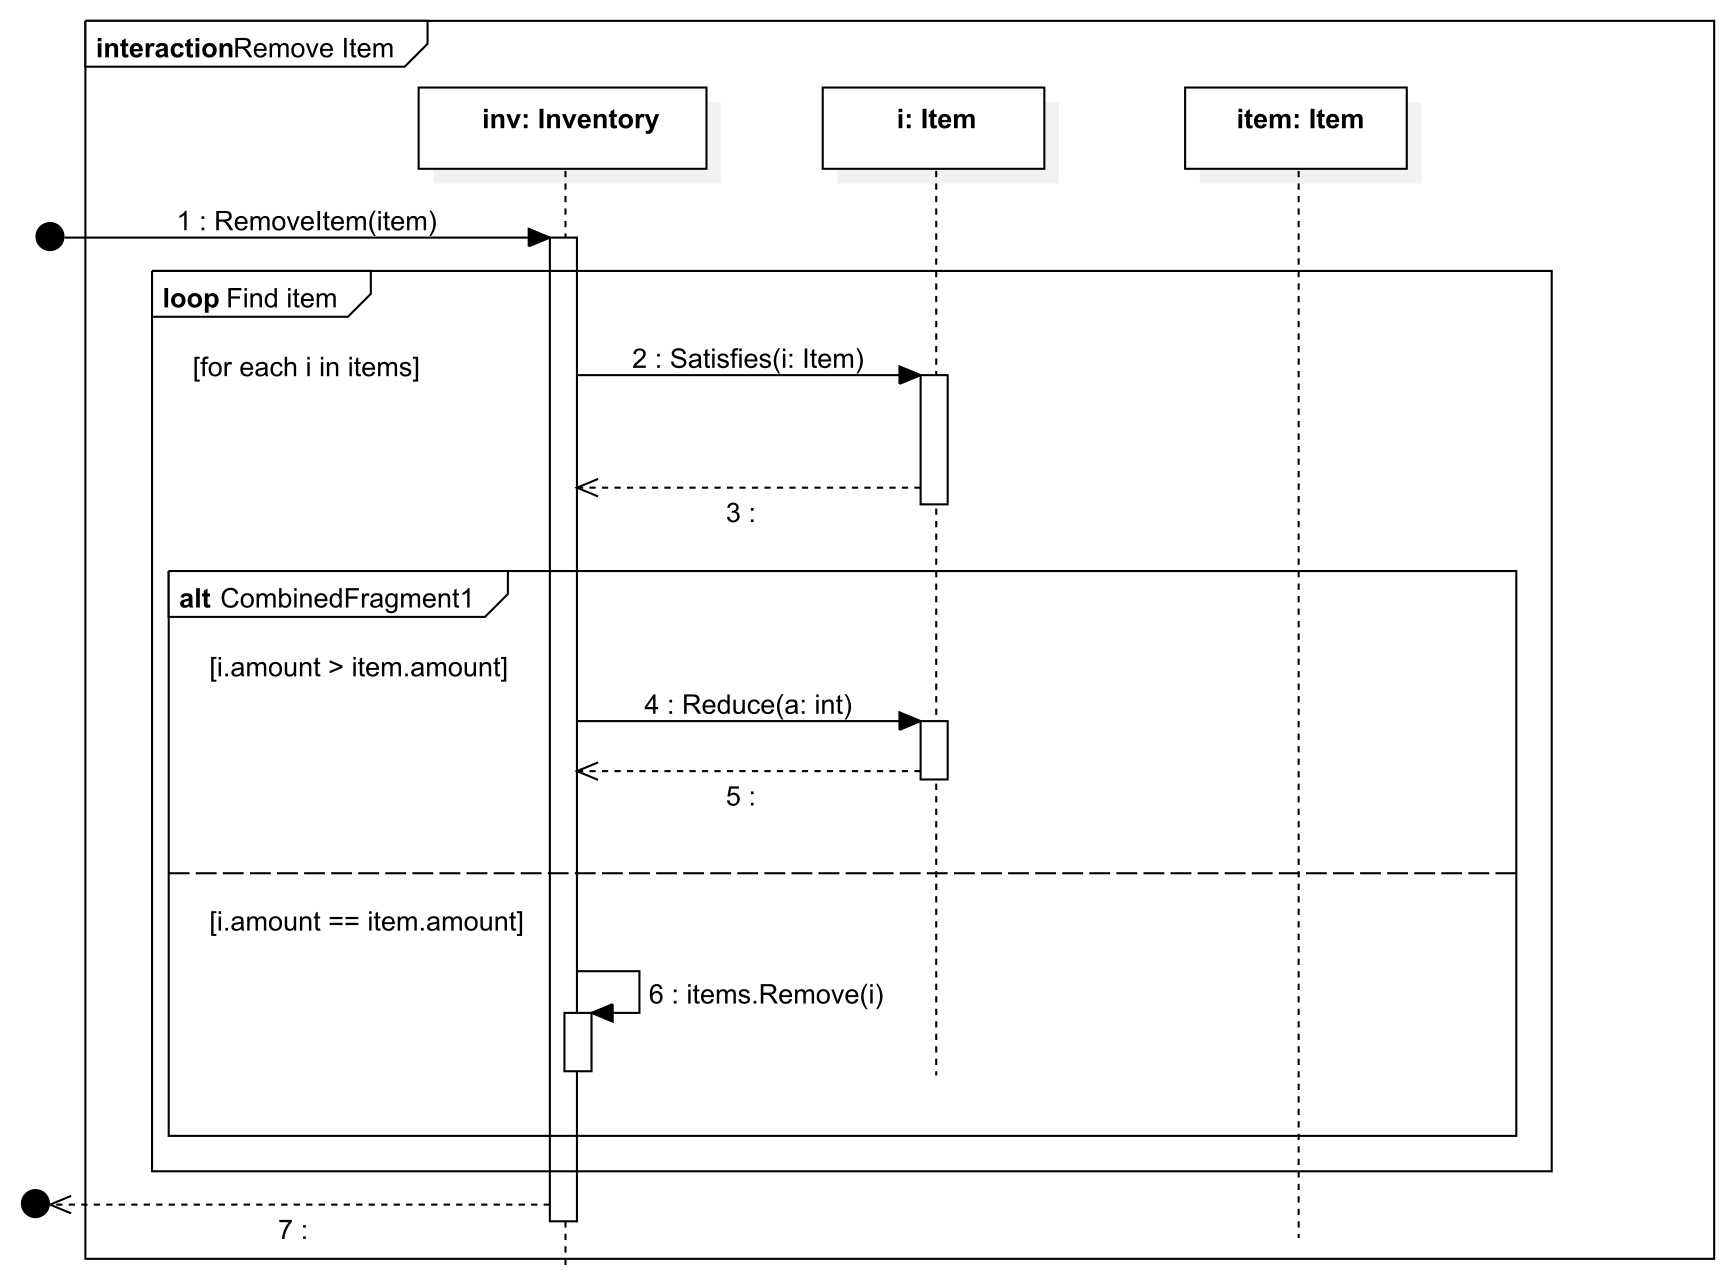
\includegraphics[width=1\textwidth]{docs/3_Project/svg/Design Model!Inventory!Remove Item!Remove Item_29.png} 
\caption{Az adott tárgyhelyből eltűnik egy vagy több egységnyi egy tárgyból.} 
\end{figure} 

\begin{figure}[H] 
\centering 
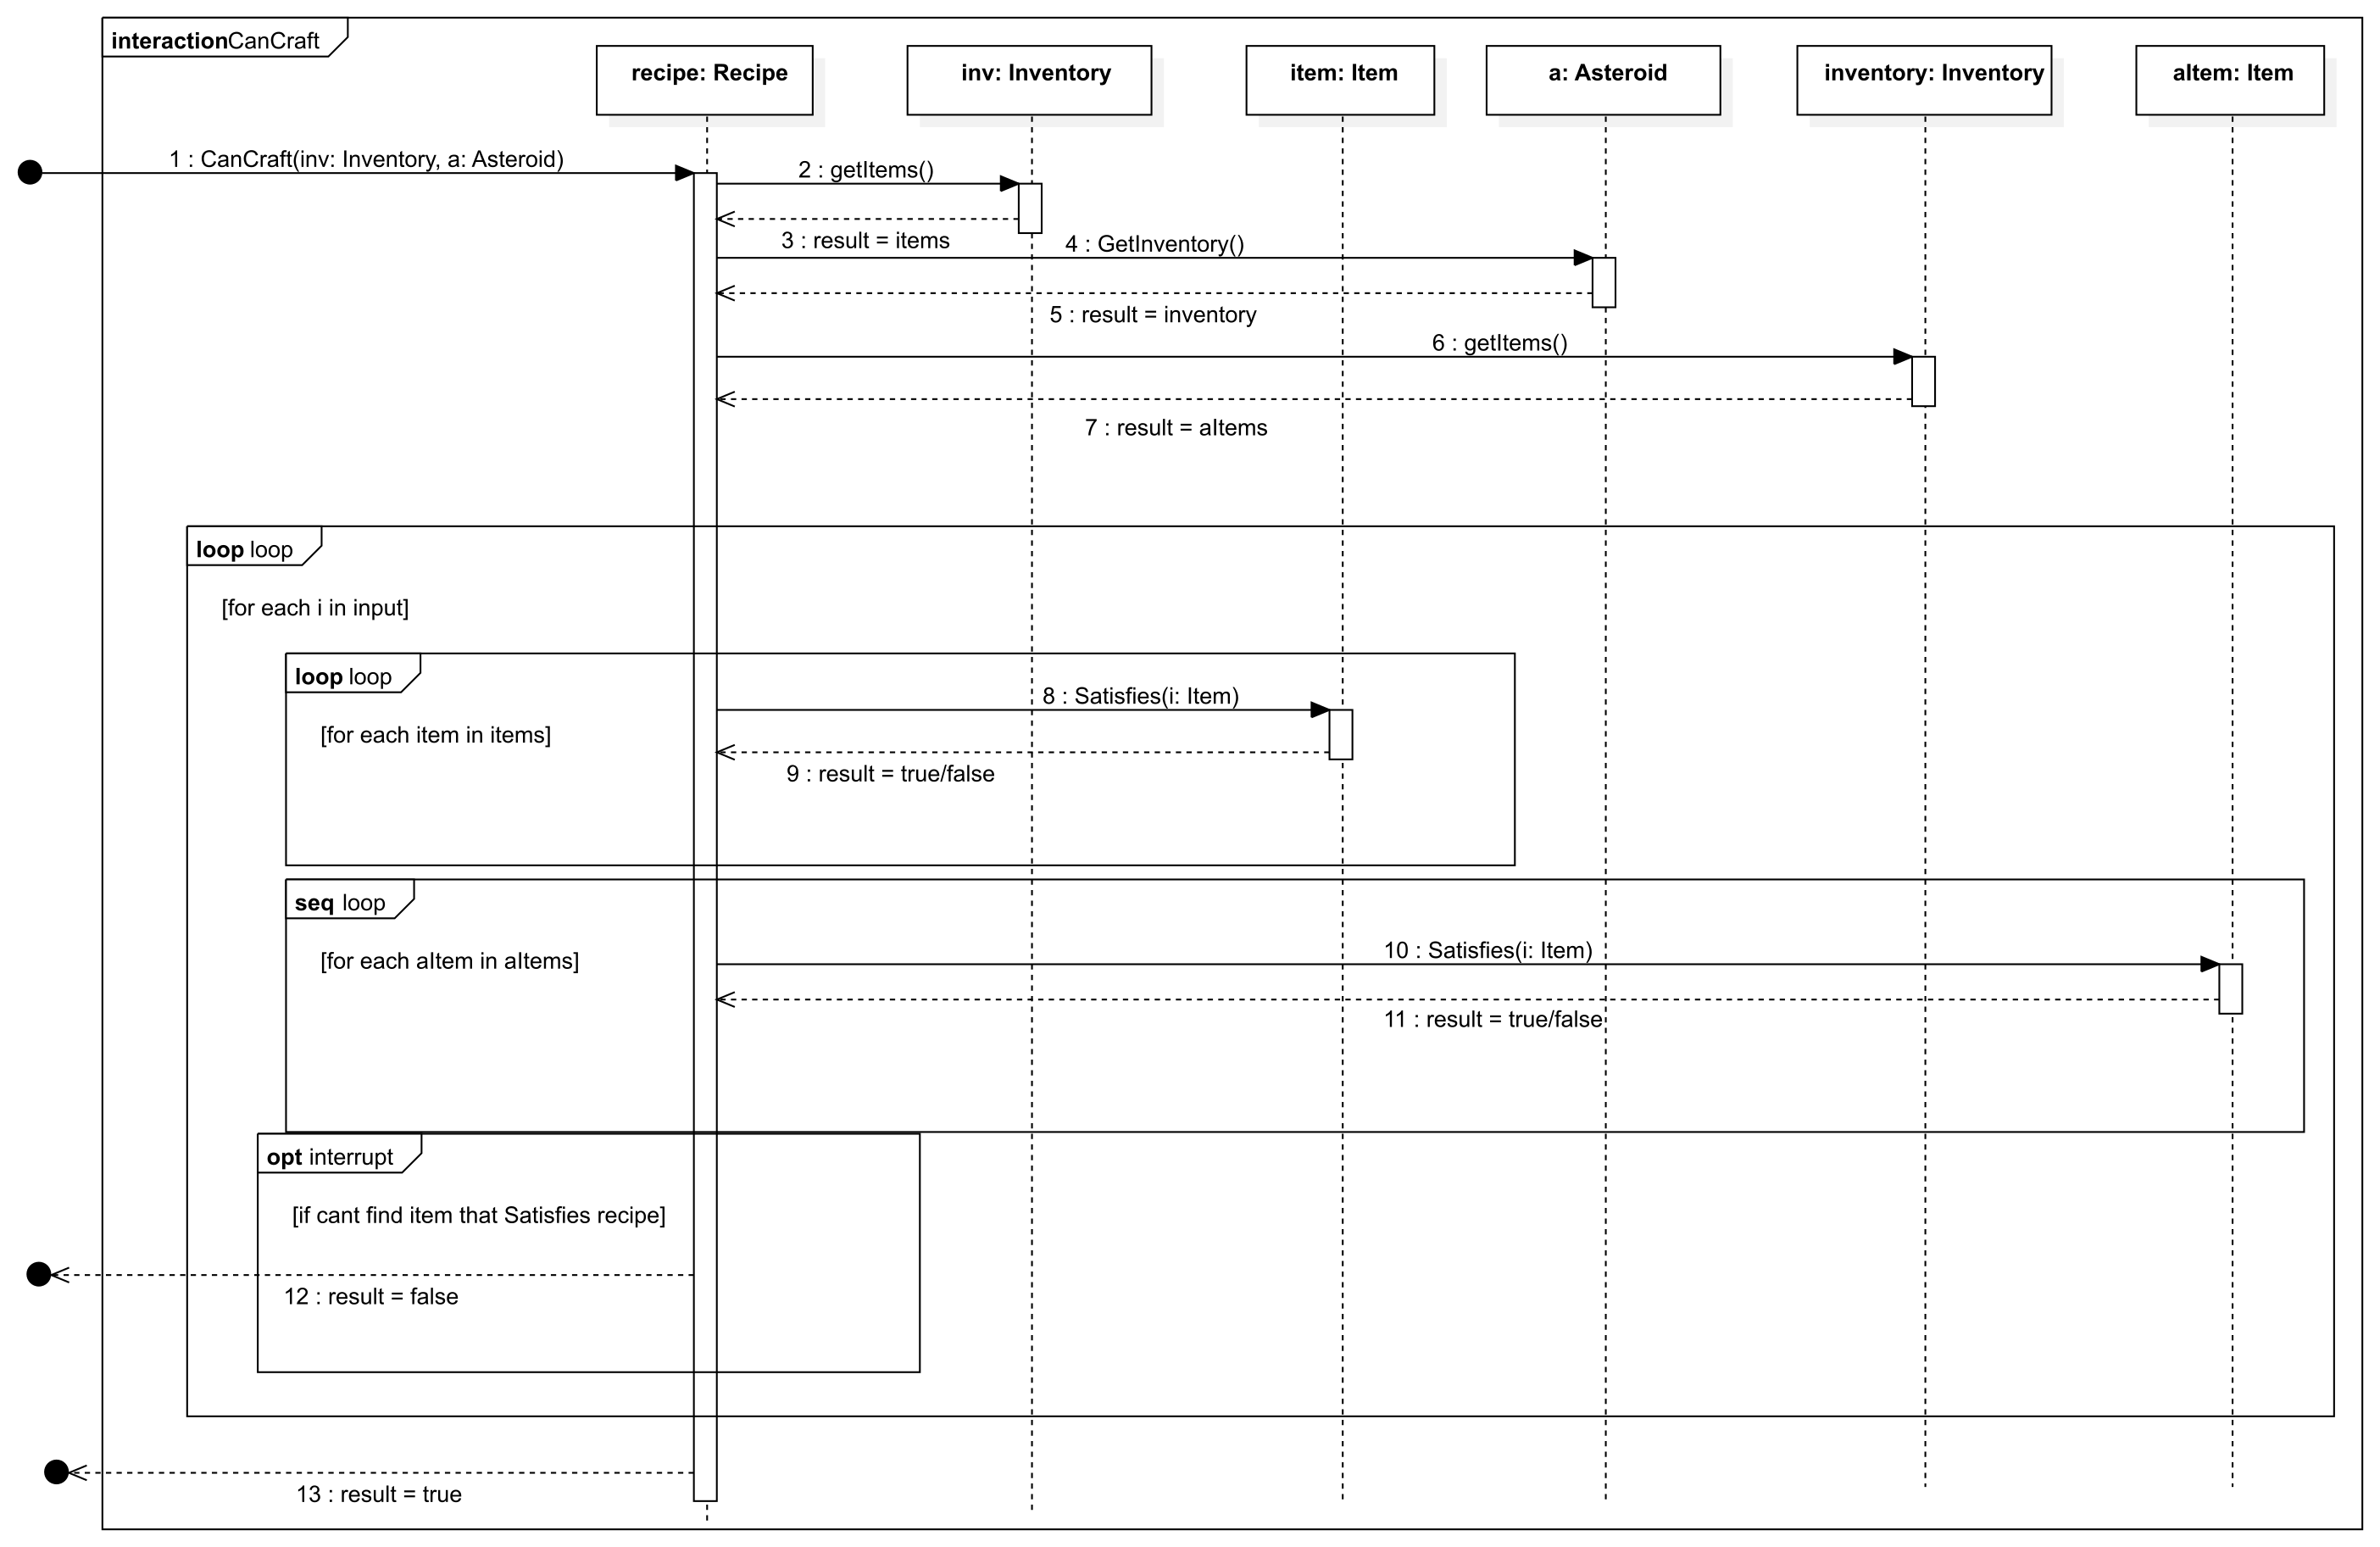
\includegraphics[width=1\textwidth]{docs/3_Project/svg/Design Model!CanCraftSeq!Can Craft!CanCraft_30.png} 
\end{figure} 

